\documentclass[review]{elsarticle}
\usepackage{lineno}
\usepackage{xspace}
\modulolinenumbers[5]

\journal{Annals of Nuclear Energy}

%% `Elsevier LaTeX' style

%%%%%%%%%%%%%%%%%%%%%%%

%%%% packages and definitions (optional)
\usepackage{placeins}
\usepackage{booktabs} % nice rules (thick lines) for tables
\usepackage{microtype} % improves typography for PDF
\usepackage{hhline}
\usepackage{amsmath}
\usepackage{mathrsfs}
\usepackage{rotating}
\usepackage{multirow}
\usepackage{mathtools}
\usepackage{amssymb}
\usepackage{slashbox}
\newcommand{\abs}[1]{\left\lvert #1 \right\rvert}
%\usepackage{adjustbox}
%\usepackage{cite}
%\usepackage[demo]{graphicx}
%\usepackage{caption}
%\usepackage{subcaption}

\usepackage{booktabs}
\usepackage{threeparttable, tablefootnote}

\usepackage{tabularx}
\newcolumntype{b}{>{\hsize=1.0\hsize}X}
\newcolumntype{s}{>{\hsize=.5\hsize}X}
\newcolumntype{m}{>{\hsize=.75\hsize}X}
\newcolumntype{x}{>{\hsize=.25\hsize}X}

\graphicspath{{figures/}}

% tikz %
\usepackage{tikz}
\usetikzlibrary{positioning, arrows, decorations, shapes}

\usetikzlibrary{shapes.geometric,arrows}
\tikzstyle{process} = [rectangle, rounded corners, minimum width=3cm, minimum height=1cm,text centered, draw=black, fill=blue!30]
\tikzstyle{object} = [ellipse, rounded corners, minimum width=3cm, minimum height=1cm,text centered, draw=black, fill=green!30]
\tikzstyle{arrow} = [thick,->,>=stealth]

% hyperref %
\usepackage[hidelinks]{hyperref}
% after hyperref %
\usepackage{cleveref}
\usepackage{datatool}
\usepackage[acronym,toc]{glossaries}
\newacronym{<++>}{<++>}{<++>}
\newacronym[longplural={metric tons of heavy metal}]{MTHM}{MTHM}{metric ton of heavy metal}
\newacronym{ABM}{ABM}{agent-based modeling}
\newacronym{ACDIS}{ACDIS}{Program in Arms Control \& Domestic and International Security}
\newacronym{AHTR}{AHTR}{Advanced High Temperature Reactor}
\newacronym{ANDRA}{ANDRA}{Agence Nationale pour la gestion des D\'echets RAdioactifs, the French National Agency for Radioactive Waste Management}
\newacronym{ANL}{ANL}{Argonne National Laboratory}
\newacronym{ANS}{ANS}{American Nuclear Society}
\newacronym{API}{API}{application programming interface}
\newacronym{ARE}{ARE}{Aircraft Reactor Experiment}
\newacronym{ARFC}{ARFC}{Advanced Reactors and Fuel Cycles}
\newacronym{ASME}{ASME}{American Society of Mechanical Engineers}
\newacronym{ATWS}{ATWS}{Anticipated Transient Without Scram}
\newacronym{BDBE}{BDBE}{Beyond Design Basis Event}
\newacronym{BIDS}{BIDS}{Berkeley Institute for Data Science}
\newacronym{BR}{BR}{Breeding Ratio}
\newacronym{CAFCA}{CAFCA}{ Code for Advanced Fuel Cycles Assessment }
\newacronym{CAS}{CAS}{Chinese Academy of Sciences} 
\newacronym{CDTN}{CDTN}{Centro de Desenvolvimento da Tecnologia Nuclear}
\newacronym{CEA}{CEA}{Commissariat \`a l'\'Energie Atomique et aux \'Energies Alternatives}
\newacronym{CFD}{CFD}{Computational Fluid Dynamics}
\newacronym{CI}{CI}{continuous integration}
\newacronym{CNEN}{CNEN}{Comiss\~{a}o Nacional de Energia Nuclear}
\newacronym{CNERG}{CNERG}{Computational Nuclear Engineering Research Group}
\newacronym{COSI}{COSI}{Commelini-Sicard}
\newacronym{COTS}{COTS}{commercial, off-the-shelf}
\newacronym{CSNF}{CSNF}{commercial spent nuclear fuel}
\newacronym{CTAH}{CTAHs}{Coiled Tube Air Heaters}
\newacronym{CUBIT}{CUBIT}{CUBIT Geometry and Mesh Generation Toolkit}
\newacronym{CURIE}{CURIE}{Centralized Used Fuel Resource for Information Exchange}
\newacronym{DAG}{DAG}{directed acyclic graph}
\newacronym{DANESS}{DANESS}{Dynamic Analysis of Nuclear Energy System Strategies}
\newacronym{DBE}{DBE}{Design Basis Event}
\newacronym{DESAE}{DESAE}{Dynamic Analysis of Nuclear Energy Systems Strategies}
\newacronym{DHS}{DHS}{Department of Homeland Security}
\newacronym{DOE}{DOE}{Department of Energy}
\newacronym{DRACS}{DRACS}{Direct Reactor Auxiliary Cooling System}
\newacronym{DRE}{DRE}{dynamic resource exchange}
\newacronym{DSNF}{DSNF}{DOE spent nuclear fuel}
\newacronym{DYMOND}{DYMOND}{Dynamic Model of Nuclear Development }
\newacronym{EBS}{EBS}{Engineered Barrier System}
\newacronym{EDF}{EDF}{Électricité de France}
\newacronym{EDZ}{EDZ}{Excavation Disturbed Zone}
\newacronym{EFPY}{EFPY}{Effective Full-Power Years}
\newacronym{EIA}{EIA}{U.S. Energy Information Administration}
\newacronym{EPA}{EPA}{Environmental Protection Agency}
\newacronym{EPR}{EPR}{European Pressurized Reactors}
\newacronym{EP}{EP}{Engineering Physics}
\newacronym{EU}{EU}{European Union}
\newacronym{FCO}{FCO}{Fuel Cycle Options}
\newacronym{FCT}{FCT}{Fuel Cycle Technology}
\newacronym{FEHM}{FEHM}{Finite Element Heat and Mass Transfer}
\newacronym{FEPs}{FEPs}{Features, Events, and Processes}
\newacronym{FHR}{FHR}{Fluoride-Salt-Cooled High-Temperature Reactor}
\newacronym{FLiBe}{FLiBe}{Fluoride-Lithium-Beryllium}
\newacronym{FP}{FP}{Fission Product}
\newacronym{FTC}{FTC}{Fuel Temperature Coefficient}
\newacronym{GDSE}{GDSE}{Generic Disposal System Environment}
\newacronym{GDSM}{GDSM}{Generic Disposal System Model}
\newacronym{GENIUSv1}{GENIUSv1}{Global Evaluation of Nuclear Infrastructure Utilization Scenarios, Version 1}
\newacronym{GENIUSv2}{GENIUSv2}{Global Evaluation of Nuclear Infrastructure Utilization Scenarios, Version 2}
\newacronym{GENIUS}{GENIUS}{Global Evaluation of Nuclear Infrastructure Utilization Scenarios}
\newacronym{GIF}{GIF}{Generation IV International Forum}
\newacronym{GPAM}{GPAM}{Generic Performance Assessment Model}
\newacronym{GRSAC}{GRSAC}{Graphite Reactor Severe Accident Code}
\newacronym{GUI}{GUI}{graphical user interface}
\newacronym{HLW}{HLW}{high level waste}
\newacronym{HPC}{HPC}{high-performance computing}
\newacronym{HTC}{HTC}{high-throughput computing}
\newacronym{HTGR}{HTGR}{High Temperature Gas-Cooled Reactor}
\newacronym{IAEA}{IAEA}{International Atomic Energy Agency}
\newacronym{IEMA}{IEMA}{Illinois Emergency Mangament Agency}
\newacronym{IHLRWM}{IHLRWM}{International High Level Radioactive Waste Management}
\newacronym{INL}{INL}{Idaho National Laboratory}
\newacronym{IHX}{IHX}{Intermediate Heat Exchanger}
\newacronym{IPRR1}{IRP-R1}{Instituto de Pesquisas Radioativas Reator 1}
\newacronym{IRP}{IRP}{Integrated Research Project}
\newacronym{ISFSI}{ISFSI}{Independent Spent Fuel Storage Installation}
\newacronym{ISRG}{ISRG}{Independent Student Research Group}
\newacronym{JFNK}{JFNK}{Jacobian-Free Newton Krylov}
\newacronym{LANL}{LANL}{Los Alamos National Laboratory}
\newacronym{LBNL}{LBNL}{Lawrence Berkeley National Laboratory}
\newacronym{LCOE}{LCOE}{levelized cost of electricity}
\newacronym{LDRD}{LDRD}{laboratory directed research and development}
\newacronym{LFR}{LFR}{Lead-Cooled Fast Reactor}
\newacronym{LLNL}{LLNL}{Lawrence Livermore National Laboratory}
\newacronym{LMFBR}{LMFBR}{Liquid Metal Fast Breeder Reactor}
\newacronym{LOFC}{LOFC}{Loss of Forced Cooling}
\newacronym{LOHS}{LOHS}{Loss of Heat Sink}
\newacronym{LOLA}{LOLA}{Loss of Large Area}
\newacronym{LP}{LP}{linear program}
\newacronym{LWR}{LWR}{Light Water Reactor}
\newacronym{MAGNOX}{MAGNOX}{Magnesium Alloy Graphie Moderated Gas Cooled Uranium Oxide Reactor}
\newacronym{MA}{MA}{minor actinide}
\newacronym{MCNP}{MCNP}{Monte Carlo N-Particle code}
\newacronym{MILP}{MILP}{mixed-integer linear program}
\newacronym{MIT}{MIT}{the Massachusetts Institute of Technology}
\newacronym{MOAB}{MOAB}{Mesh-Oriented datABase}
\newacronym{MOOSE}{MOOSE}{Multiphysics Object-Oriented Simulation Environment}
\newacronym{MOSART}{MOSART}{Molten Salt Actinide Recycler and Transmuter}
\newacronym{MOX}{MOX}{mixed oxide}
\newacronym{MPI}{MPI}{Message Passing Interface}
\newacronym{MRPP}{MRPP}{Multiregion Processing Plant}
\newacronym{MSBR}{MSBR}{Molten Salt Breeder Reactor}
\newacronym{MSFR}{MSFR}{Molten Salt Fast Reactor}
\newacronym{MSRE}{MSRE}{Molten Salt Reactor Experiment}
\newacronym{MSR}{MSR}{Molten Salt Reactor}
\newacronym{MTC}{MTC}{Moderator Temperature Coefficient}
\newacronym{NAGRA}{NAGRA}{National Cooperative for the Disposal of Radioactive Waste}
\newacronym{NEAMS}{NEAMS}{Nuclear Engineering Advanced Modeling and Simulation}
\newacronym{NEUP}{NEUP}{Nuclear Energy University Programs}
\newacronym{NFCSim}{NFCSim}{Nuclear Fuel Cycle Simulator}
\newacronym{NGNP}{NGNP}{Next Generation Nuclear Plant}
\newacronym{NMWPC}{NMWPC}{Nuclear MW Per Capita}
\newacronym{NNSA}{NNSA}{National Nuclear Security Administration}
\newacronym{NPP}{NPP}{Nuclear Power Plant}
\newacronym{NPRE}{NPRE}{Department of Nuclear, Plasma, and Radiological Engineering}
\newacronym{NQA1}{NQA-1}{Nuclear Quality Assurance - 1}
\newacronym{NRC}{NRC}{Nuclear Regulatory Commission}
\newacronym{NSF}{NSF}{National Science Foundation}
\newacronym{NSSC}{NSSC}{Nuclear Science and Security Consortium}
\newacronym{NUWASTE}{NUWASTE}{Nuclear Waste Assessment System for Technical Evaluation}
\newacronym{NWF}{NWF}{Nuclear Waste Fund}
\newacronym{NWTRB}{NWTRB}{Nuclear Waste Technical Review Board}
\newacronym{OCRWM}{OCRWM}{Office of Civilian Radioactive Waste Management}
\newacronym{ORION}{ORION}{ORION}
\newacronym{ORNL}{ORNL}{Oak Ridge National Laboratory}
\newacronym{PARCS}{PARCS}{Purdue Advanced Reactor Core Simulator}
\newacronym{PBAHTR}{PB-AHTR}{Pebble Bed Advanced High Temperature Reactor}
\newacronym{PBFHR}{PB-FHR}{Pebble-Bed Fluoride-Salt-Cooled High-Temperature Reactor}
\newacronym{PEI}{PEI}{Peak Environmental Impact}
\newacronym{PH}{PRONGHORN}{PRONGHORN}
\newacronym{PRIS}{PRIS}{Power Reactor Information System}
\newacronym{PRKE}{PRKE}{Point Reactor Kinetics Equations}
\newacronym{PSPG}{PSPG}{Pressure-Stabilizing/Petrov-Galerkin}
\newacronym{PWAR}{PWAR}{Pratt and Whitney Aircraft Reactor}
\newacronym{PWR}{PWR}{Pressurized Water Reactor}
\newacronym{PyNE}{PyNE}{Python toolkit for Nuclear Engineering}
\newacronym{PyRK}{PyRK}{Python for Reactor Kinetics}
\newacronym{QA}{QA}{quality assurance}
\newacronym{RDD}{RD\&D}{Research Development and Demonstration}
\newacronym{RD}{R\&D}{Research and Development}
\newacronym{REE}{REE}{rare earth element}
\newacronym{RELAP}{RELAP}{Reactor Excursion and Leak Analysis Program}
\newacronym{RIA}{RIA}{Reactivity Insertion Accident}
\newacronym{RIF}{RIF}{Region-Institution-Facility}
\newacronym{ROD}{ROD}{Reactor Optimum Design}
\newacronym{SD-TMSR}{SD-TMSR}{Single-fluid Double-zone Thorium-based Molten Salt Reactor}	
\newacronym{SFR}{SFR}{Sodium-Cooled Fast Reactor}
\newacronym{SINDAG}{SINDA{\textbackslash}G}{Systems Improved Numerical Differencing Analyzer $\backslash$ Gaski}
\newacronym{SKB}{SKB}{Svensk K\"{a}rnbr\"{a}nslehantering AB}
\newacronym{SNF}{SNF}{spent nuclear fuel}
\newacronym{SNL}{SNL}{Sandia National Laboratory}
\newacronym{STC}{STC}{specific temperature change}
\newacronym{SUPG}{SUPG}{Streamline-Upwind/Petrov-Galerkin}
\newacronym{SWF}{SWF}{Separations and Waste Forms}
\newacronym{SWU}{SWU}{Separative Work Unit}
\newacronym{TRIGA}{TRIGA}{Training Research Isotope General Atomic}
\newacronym{TRISO}{TRISO}{Tristructural Isotropic}
\newacronym{TSM}{TSM}{Total System Model}
\newacronym{TSPA}{TSPA}{Total System Performance Assessment for the Yucca Mountain License Application}
\newacronym{ThOX}{ThOX}{thorium oxide}
\newacronym{UFD}{UFD}{Used Fuel Disposition}
\newacronym{UML}{UML}{Unified Modeling Language}
\newacronym{UOX}{UOX}{uranium oxide}
\newacronym{UQ}{UQ}{uncertainty quantification}
\newacronym{US}{US}{United States}
\newacronym{UW}{UW}{University of Wisconsin}
\newacronym{VISION}{VISION}{the Verifiable Fuel Cycle Simulation Model}
\newacronym{VVER}{VVER}{Voda-Vodyanoi Energetichesky Reaktor (Russian Pressurized Water Reactor)}
\newacronym{VV}{V\&V}{verification and validation}
\newacronym{WIPP}{WIPP}{Waste Isolation Pilot Plant}
\newacronym{YMR}{YMR}{Yucca Mountain Repository Site}
\newacronym{CNRS}{CNRS}{National Center for Scientific Research}		
\newacronym{CRAM}{CRAM}{Chebyshev Rational Approximation Method}
\newacronym{DT}{DT}{Doubling Time}		
\newacronym{Euratom}{Euratom}{European Atomic Energy Community}
\newacronym{FPs}{FPs}{Fission Products} 
\newacronym{HM}{HM}{Heavy Metal}
\newacronym{MAs}{MAs}{Minor Actinides}
\newacronym{OpenMP}{OpenMP}{Open Multi-Processing}
\newacronym{TCR}{TCR}{Temperature Coefficient of Reactivity}
\newacronym{3D}{3D}{Three Dimensions}			
\newacronym{TS-MSR}{TS-MSR}{Thermal-Spectrum Molten Salt Reactor}
\newacronym{FS-MSR}{FS-MSR}{Fast-Spectrum Molten Salt Reactor}
\newacronym{EVOL}{EVOL}{Evaluation and Viability of Liquid Fuel Fast Reactor System}
\newacronym{TMSR}{TMSR}{Thorium Molten Salt Reactor}


\makeglossaries

\begin{document}
\begin{frontmatter}
\title{Various scenarios for transition to thorium fuel cycle in the Single-fluid Double-zone Thorium Molten Salt Reactor (SD-TMSR)}

\date{}                     %% if you don't need date to appear

%% Authors
\author[mephi,shams]{O. Ashraf\corref{corrauthor}}
\cortext[corrauthor]{Corresponding Author}
\ead{osama.ashraf@edu.asu.edu.eg}
\author[uiuc]{Andrei Rykhlevskii}
%\author[mephi]{Anton Smirnov}
\author[mephi]{G. V. Tikhomirov}
\author[uiuc]{Kathryn D. Huff} %



% Institutes of the authors
\address[mephi]{Dept. of Theoretical and Experimental Physics of Nuclear Reactors, Institute of Nuclear Physics and Engineering, National Research Nuclear University MEPhI, 31, Kashirskoe Shosse, Moscow, 115409, Russian Federation}
\address[shams]{Physics Department, Faculty of Education, Ain Shams University, Cairo, Egypt, 11341}
\address[uiuc]{Dept. of Nuclear, Plasma, and Radiological Engineering, University of Illinois at Urbana-Champaign, Urbana, IL 61801, United States}

	
\begin{keyword}
MSR \sep
thorium fuel cycle \sep
transmuter \sep
burner \sep
online reprocessing \sep
Monte carlo code
%moderated molten salt reactor \sep
%single-fluid double-zone thorium molten salt reactor \sep
%sd-tmsr \sep
%nuclear fuel cycle \sep
%salt treatment
\end{keyword}


\begin{abstract}
Liquid-fueled \gls{MSR} systems represent advances in safety, economics, sustainability, and proliferation resistance. The \gls{MSR} has been designed to operate with a Th/$^{233}$U fuel cycle with $^{233}$U used as startup fissile material. Since $^{233}$U does not exist in nature, we must examine other available fissile materials to start up these reactor concepts. This work investigates the fuel cycle and neutronics performance of the \gls{SD-TMSR} with different fissile material loadings at startup: \gls{HALEU} (19.79\%), Pu mixed with \gls{LEU} (19.79\%), reactor-grade Pu (a mixture of Pu isotopes chemically extracted from \gls{PWR} \gls{SNF} with $33$ $GWd/tHM$ burnup), \gls{TRU} from \gls{LWR} \gls{SNF}, and $^{233}$U.
The \gls{MSR} burnup routine provided by SERPENT-2 is used to simulate the online reprocessing and refueling in the \gls{SD-TMSR}. The effective multiplication factor, fuel salt composition evolution, and net production of $^{233}$U are studied in the present work. Additionally, the neutron spectrum shift during the reactor operation is calculated. The results show that the continuous flow of reactor-grade Pu helps transition to the thorium fuel cycle within a relatively short time ($\approx$ $4.5$ years) compared to $26$ years for $^{233}$U startup fuel. Finally, using \gls{TRU} as the initial fuel materials offers the possibility of operating the SD-TMSR for an extended period of time ($\approx$ $40$ years) without any external feed of $^{233}$U.
\end{abstract}

\end{frontmatter}
\glsresetall

\linenumbers

%\printglossary[type=\acronymtype,title=Abbreviations]

\section{Introduction}
The \gls{GIF} has defined eight technology goals for the next generation
nuclear systems. These goals are: safety and reliability, economics,
sustainability, non-proliferation and physical protection
\cite{doe2002technology}. The \gls{MSR} has many advantages that consistent
with \gls{GIF}'s goals, for example, liquid fuel, inherent safety, online
reprocessing and refueling, excellent neutron economy and operation near
atmospheric
pressure in a primary loop \cite{siemer2015molten,rosenthal1970molten}.
Thus, the \gls{GIF} selected \gls{MSR} as one of the promising Generation-IV
reactors \cite{doe2002technology,pioro2016handbook}.
In the \gls{MSR}, the fuel is dissolved in a molten salt (e.g., LiF or NaCl).
This liquid fuel salt (e.g., LiF-BeF$_2$-ThF$_4$-$^{233}$UF$_4$) constantly
circulates through the core and allows transferring fission heat from reactor
core to heat exchanger.

The Single-fluid Double-zone Thorium-based Molten Salt Reactor (SD-TMSR-2,250
MW$_{th}$) was introduced by the \gls{CAS} \cite{li_optimization_2018}. The
SD-TMSR
is a graphite-moderated thermal-spectrum \gls{MSR} operating in Th/$^{233}$U
fuel cycle. In the SD-TMSR the fissile and fertile elements are integrated
into the same salt. In addition, the active core is divided into two zones,
the radius of the fuel channels in the outer zone is modified to be larger
than the radius of the fuel channels in the inner zone to improve the breeding
ratio \cite{nuttin2005potential,li_optimization_2018}.

Historically, the thermal-spectrum \gls{MSR} was designed for the Th/$^{233}$U
fuel cycle \cite{rykhlevskii2019modeling,nuttin2005potential,
merle2004scenarios,rosenthal1970molten}. This design assumes that we have
fissile $^{233}$U inventory to startup new \glspl{MSR}. But $^{233}$U does not
exist in the Earth's crust and can be produced from fertile $^{232}$Th only in
the nuclear reactor. Therefore, it is required to examine alternative fissile
materials (e.g., $^{235}$U) to replace the $^{233}$U in the startup fuel
composition \cite{betzler2016modeling,zou2018transition}. The thorium fuel
cycle transition can be achieved after reaching the doubling
time\footnote{Time required to produce enough amount of $^{233}$U to trigger a
new SD-TMSR.} of $^{233}$U because in this case all startup fissile material
is being substituted by newly produced $^{233}$U.

Betzler \emph{et al.} discussed the simulation of the startup of a MSBR unit
cell with \gls{LEU} (19.79\%) and Pu from \gls{LWR} spent fuel (SF) as initial
fissile materials \cite{betzler2016modeling}. They concluded that the 
plutonium vector extracted from LWR SF is the best alternative source to 
$^{233}$U because it has the highest ratio of fissile isotopes
\cite{betzler2016modeling}. Zou \emph{et al.} introduced two approaches for
the thorium fuel cycle transition in \gls{TMSR}: (1) in-core transition and 
(2) ex-core transition. In the first approach, the TMSR is launched with 
existing fissile material and thorium as a fertile material; then the 
$^{233}$U bred from thorium is rerouted into the core to maintain criticality. 
In contrast, the second approache tends to store produced $^{233}$U out of the 
core until there is enough amount to start a new TMSR \cite{zou2018transition}.
Additionally, Zou \emph{et al.} studied the transitioning to thorium fuel
cycle in a small modular Th-based molten salt reactor (smTMSR) using \gls{TRU}
as startup fuel. They concluded that the transition to thorium fuel cycle can
be achieved in thermal smTMSR with a proper fuel fraction 
\cite{zou2018preliminary}.

Heuer \emph{et al.} discussed the transition characteristics of the \gls{MSFR}
under different launching scenarios (e.g., enriched uranium and TRU)
\cite{heuer2014towards}.

Indeed, there are various researches that revolve around starting the
\glspl{MSR} with fissile materials alternative to $^{233}$U. Many of these
researches focus on the fast-spectrum \glspl{MSR} \cite{ashraf2019modeling,
ashraf2018nuclear, rykhlevskii_fuel_2019, betzler_impacts_2019,
heuer2014towards,fiorina2013investigation}, while little focus on
thermal-spectrum \glspl{MSR} \cite{betzler2016modeling, zou2018preliminary,
zou2018transition}. Nevertheless, starting the \gls{SD-TMSR} with other
fissile materials (except $^{233}$U) was not studied before. Therefore,
the main object of the present paper is to discuss the simulation of the
\gls{SD-TMSR} operation for a lifetime-long period of time (60 years) with
different initial fissile materials and without any external feed of $^{233}$U
to achieve the thorium fuel cycle transition. We investigated five different
initial fissile materials: \gls{LEU}, Pu, and \gls{TRU} from LWR SF
\cite{de2000scenarios}. Moreover, two different feed scenarios were selected:
\begin{itemize}
	\item Continuous feed flow of thorium and $^{233}$U from \texttt{Pa-decay tank}, where the removal rate of $^{233}$Pa = feed rate of $^{233}$U. \cite{betzler2016modeling}.
	\item Continuous feed flow of (Heavy Metal (HM) except for Th) + all or part of $^{233}$U from \texttt{Pa-decay tank}.
\end{itemize}
This present paper is organized as follows: after an introduction about \gls{MSR} systems, the model description is discussed in section 2. Methodology and tools is descried in section 3. Extraction and feed mechanisms are addressed in section 4. Section 5 focuses on the results and discussion. Finally, section 6 highlights the conclusions.

%produce enough amount of $^{233}$U to start a new \gls{SD-TMSR}.
%Therefore, the aim of this paper is to operate the \gls{SD-TMSR} for a long period of time with different initial fissile materials without external feed of $^{233}$U (that does not exist anywhere) to produce enough amount of $^{233}$U that is required to start a new \gls{SD-TMSR}.


%The \gls{MSR} is the only liquid-fueled reactor that the \gls{GIF} has chosen as one of the six promising concepts \cite{doe2002technology,pioro2016handbook}. The reactor's liquid fuel distinguishes it from other nuclear reactors. \glspl{MSR} can operate extended time without shutdown for refueling with a superior neutron economy \cite{doe2002technology}. Introducing online reprocessing and refueling systems would ensure sustainability. In a \gls{MSR}, liquid fuel salt (e.g. a mixture of LiF-BeF$_2$-ThF$_4$-$^{233}$UF$_4$) circulates through the core and transports fission heat to the \glspl{IHX}. Finally, this type of reactor has a high conversion efficiency and a negative temperature coefficient.

%Both thermal and fast \gls{MSR} concepts exist in the literature \cite{pioro2016handbook,engel1979development}. For thermal \glspl{MSR}, hexagonal graphite prisms act as moderators. In contrast, fast spectrum \glspl{MSR} lack moderators. A \gls{MSR} can breed in both cases, making them optimal for realizing a desirable Thorium-Uranium fuel cycle \cite{hargraves2010liquid}.

%In the 1950s, \gls{ORNL} performed experiments that provided a basis for \gls{MSR} feasibility. In 1958, a 5 MW$_{th}$ homogeneous reactor experiment called HRE-2 utilized water-based liquid fuel to illustrate the intrinsic stability of homogeneous reactors. In the 1960s, \gls{ORNL} performed the \gls{MSRE} \cite{engel1979development,haubenreich1970experience,fiorinibasis,robertson1965msre}. These experiments demonstrated the capability of circulating a liquid fluoride mixture without significant corrosion problems. Researchers used a nickel-based alloy (Hastelloy N) as structural material and controlled the fuel's oxidation by using a U$^{3+}$/U$^{4+}$ buffer. The experiment also tested the continuous reprocessing of liquid fuel. The results showed that introducing a noble gas system (i.e. gas bubbling system) during the fuel cycle helps extract gaseous fission products \cite{pioro2016handbook}.

%\gls{ORNL} later researched the \gls{MSBR} \cite{rosenthal1970molten}. There were two types of \gls{MSBR}: the single-fluid molten salt reactor and the two-fluid molten salt reactor. While the single-fluid MSR dissolves fertile and fissile materials in the same salt, the two-fluid MSR physically separates them. The two-fluid MSR had a higher breeding performance than the single-fluid MSR. However, the single-fluid MSR can operate as an iso-breeding reactor as long as there is an efficient reprocessing system for the fuel salt \cite{rosenthal1970molten}.

%Despite the success of the \gls{MSRE}, \gls{ORNL} halted work on the \gls{MSBR} in 1976. The \gls{Euratom} later revived the project. To enhance the breeding performance of the \gls{MSBR}, \gls{Euratom} introduced the idea of dividing the core into multiple zones of fuel channels with different radii \cite{nuttin2005potential}. The results showed that increasing the radii of the outer fuel channels relative to the inner radii improved the reactor's breeding and allowed it to out-perform the reactor with a single-zone core and large fuel channels \cite{nuttin2005potential}.

%Later, fast spectrum MSRs were introduced. Several fast MSR designs include: \gls{MSFR}, \gls{EVOL} \cite{serp2014molten}, \gls{MOSART} \cite{boussier2012molten}, REBUS-3700 \cite{mourogov2006potentialities} and Molten Chloride Salt Fast Reactor \cite{taube1978fast}. \gls{GIF} has elected to further research \gls{MSFR} and \gls{MOSART} \cite{serp2014molten,boussier2012molten,locatelli2013generation,pettersen2016coupled}. Both designs feature the fast-spectrum, Th-based fuel, and liquid fuel circulation. The \gls{MSFR} concept initially gained momentum at \gls{CNRS} in France, and the \gls{MOSART} concept is in progress in Russia.

%Indeed, several challenges interfere with the commercial adoption of \gls{MSFR}. For example, large initial inventory of $^{233}$U and relatively long doubling time for $^{233}$U production. Moreover, material scientists must identify or create structural materials which have reasonable lifespan in extreme operational conditions (high temperature, large neutron flux, chemically aggressive salt). Finally, breeding of high-quiality fissile material in the \gls{MSFR} blanket rises significant nuclear non-proliferation concerns \cite{pettersen2016coupled,merle2009minimizing}.

%The thermal MSR has priority due to the low inventory of initial fissile $^{233}$U and short doubling time for its production \cite{ZOU2015114}.
%Nagy et al. studied the effect of core zoning on the breeding performance and graphite lifespan of a graphite-moderated MSR \cite{nagy2011new,nagy2012effects}. Li et al. divided the active core into two zones to improve the breeding performance \cite{li_optimization_2018}. The central zone is moderated, while the unmoderated outer zone acts as a subcritical fast spectrum zone \cite{li_optimization_2018}.

%In 2011, the \gls{CAS} established the strategic project ``Future Advanced Nuclear Energy $-$ Thorium-based Molten Salt Reactor System (TMSR)". Since then, several studies aimed to improve the \gls{TMSR} to efficiently utilize the Th-U fuel cycle \cite{li_optimization_2018,jiang2012advanced,li2015analysis,li2017model}.
%Separately, we can highlight the issue of a closed Th-U fuel cycle in the thermal spectrum. A number of studies have shown the fundamental possibility of organizing such a cycle in a heavy-water reactor and referred to the limitation of the burn-up of solid fuels due to the accumulation of the fission products (FPs) \cite{dastur1995thorium,bergel2004mode,bergelson2008op}. The question of feasibility and parameters of a closed U-Th fuel cycle in a \gls{TMSR} reactor is relevant.

%Liquid-fueled systems require specific neutron transport and depletion tools that capture online fuel reprocessing and refueling. Specifically, the circulation of the liquid fuel and the continuous feed or removal of elements (e.g. fissile material injection into and Fission Products (FPs) extraction from the fuel salt) are out-of-scope for most contemporary nuclear reactor physics software, which was originally written primarily to simulate solid-fueled reactors. The SERPENT-2 \cite{leppanen2014serpent} code extension takes into account the online fuel reprocessing and its effects on depletion calculations \cite{aufiero2013extended}.

%The present paper aims to analyze the fuel depletion of the \gls{SD-TMSR} during 60 years reactor operation time using SERPENT-2. This work investigates the inventory of isotopes in the core to establish the advantages of the \gls{TMSR} concept applied to energy production (based on the thorium fuel cycle). All calculations presented in the present work were implemented using SERPENT-2 version 2.1.30. We adopted the built-in SERPENT-2 subroutine to simulate continuous online reprocessing and refueling in contrast with other batch-wise codes \footnote{In the batch-wise technique, the simulation stops at a certain time and restarts after removing of poisoning isotopes and addition of fissile and/or fertile materials.} (e.g. SaltProc \cite{rykhlevskii2019modeling} and MCNP6-PYTHON \cite{Jeong2016}).
%SERPENT-2 allowed us to conduct burn-up calculations on computer clusters with multiple cores using distributed-memory MPI parallelization. The drift of the delayed neutron precursors is not examined in this paper.

%The present paper is organized as follows: after a general introduction about \gls{MSR} systems, section 2 briefly presents the \gls{SD-TMSR}. Section 3 focuses on the methodology and calculation tools used in this work. Fission products extraction modeling is described in section 4. Section 5 highlights the results and discussion. Finally, section 6 summarizes the conclusions.

% State the objectives of the work and provide an adequate background, avoiding
% a detailed literature survey or a summary of the results.

\FloatBarrier
\section{Model description} \label{Model-description}
\subsection{Geometry}
The SD-TMSR design model was introduced by the Chinese Academy of Sciences as a part of  
the strategic project ``Thorium-based Molten-Salt Reactor(TMSR) nuclear energy system" 
\cite{jiang2012advanced,li2015analysis,li_optimization_2018}. The 
design of the SD-TMSR is inspired by the \gls{MSBR} 
\cite{robertson_conceptual_1971} after modifying the geometry to 
control the positive moderator temperature coefficient in the MSBR. Li \emph{et al.} and Ashraf \emph{et al.} 
described the SD-TMSR core 
geometry in \cite{li_optimization_2018,ashraf2019whole_core}. 
Figure~\ref{fig:ff} illustrates the quarter-core view of the 
SD-TMSR.
The active zone is a right cylinder with height and diameter 
equal to 460 cm. Assemblies of graphite\footnote{We choose graphite density of 
$2.3$ g/cm$^3$, to validate our results against results in literature 
\cite{li_optimization_2018,nuttin2005potential}.} hexagonal prisms fill the 
core. The optimal side length of the graphite hexagonal prism was found in previous work to be 7.5 cm \cite{li_optimization_2018}. The liquid fuel circulates 
continuously through fuel channels that pierce the graphite hexagonal 
prisms. Two radial zones divide the core to enhance 
Th/$^{233}$U breeding performance; the radii of the fuel channels in the 
outer and inner zone are 5 and 3.5 cm, respectively. The axial and radial 
graphite reflectors surround the core to minimize neutron leakage and 
maximize flux in the core. B${_4}$C cylinder surrounds the reflectors and 
acts as radiation shielding. The SD-TMSR pressure vessel is made of a Ni-based (hastelloy N) alloy holds 
the fuel salt, graphite elements, reflector, shielding, and intermediate heat exchanger. The main 
characteristics of the SD-TMSR are listed in Table~\ref{tab:table1}.

\begin{figure} % replace 't' with 'b' to \centering [hbp!]
	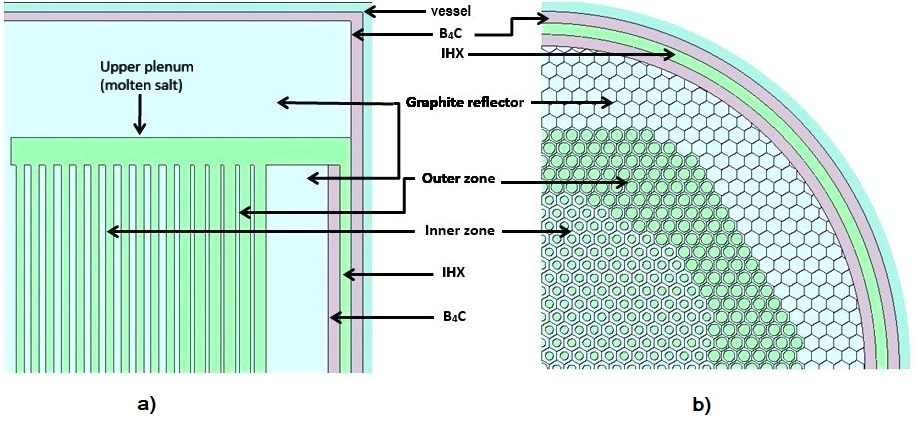
\includegraphics[width=\textwidth]{ff.png}
	\caption{$XZ$ (a) and $XY$ (b) section of the quarter-core model of the 
	SD-TMSR \cite{ashraf2019Preliminary}.}
	\label{fig:ff}
\end{figure}

\begin{table}  %[!ht]
	\caption{The main characteristics of the SD-TMSR \cite{li_optimization_2018,ashraf2019whole_core}.}
	\vspace{0.1in}
	\begin{tabularx}{\textwidth}{l | r}
		\hline
		Thermal power, MW$_{th}$          				&  2,250  \\ 
		Fuel salt components                            & LiF-BeF$_2$-(\gls{HM})F$_N$ \\
		Fuel composition, mole\%                        & 70-17.5-12.5    \\
		$^7$Li enrichment, \%        				& 99.995   \\
		Fuel temperature, K 							& 900  \\
		Fuel density at 900 K, g/cm$^3$		  		& 3.3 \\
		Fuel dilatation coefficient, g/(cm$^3$$.$K)  &  -6.7$\times$10$^{-4}$ \\
		Graphite density, g/cm$^3$             	    & 2.3	\\  
		B$_4$C density, g/cm$^3$					& 2.52  \\
		$^{10}$B enrichment, \%						&  18.4  \\
		Core diameter, cm								& 460  \\
		Core height, cm									& 460  \\
		Side length of the graphite hexagonal prism, cm   & 7.5 \\
		Inner radius, cm							& 3.5  \\
		Outer radius, cm							& 5  \\
		Ratio of molten salt and graphite in the inner zone	&  0.357  \\
		Ratio of molten salt and graphite in the outer zone &  1.162  \\
		Fuel volume, m$^3$  &	52.9 \\
		\hline
	\end{tabularx}
	\label{tab:table1}
\end{table}

\subsection{Fuel composition}
The general composition of the startup liquid fuel salt in this work is 70LiF - 
17.5BeF$_2$ - 12.5(HM)F$_N$ mole\%, where HM is the heavy metal (mixture of 
thorium and one of these fissile materials: \gls{HALEU}, Pu mixed with \gls{HALEU}, reactor-grade Pu, \gls{TRU}, and $^{233}$U), and $N$ is dependent on the chosen fissile material and the thermochemical state of the liquid fuel salt.

The aim of this paper is to simulate the  
operation of the SD-TMSR for 60 years with various startup fissile 
compositions and without any external feed of fissile $^{233}$U which we 
assume is unavailable. For that reason, five different types of initial 
fissile materials are considered based on \gls{HALEU}, Pu, and \gls{TRU} from Light Water
Reactor (LWR) spent nuclear fuel (SNF):
\begin{enumerate}[label=(\alph*)]
	\item High Assay Low Enriched Uranium (HALEU) (19.79\%),
	\item Pu mixed with \gls{HALEU} (19.79\%),
	\item reactor-grade Pu \cite{marka1993explosive},
	\item transuranic (TRU) elements from LWR SNF \cite{de2000scenarios}, and
	\item $^{233}$U for comparison \cite{ashraf2019whole_core}.
\end{enumerate}
All types of initial fissile materials are fed as fluorides.
The reactor-grade Pu and \gls{TRU} compositions are summarized in 
Table~\ref{tab:table2} and ~\ref{tab:table3}, respectively.

\begin{table} % [!ht]
	\centering
	\caption{Reactor-grade Pu vector (wt.\%) \cite{marka1993explosive}.}
	\vspace{0.1in}
	\begin{tabularx}{\textwidth}{X X X X X}
		\hline
		$^{238}$Pu & $^{239}$Pu & $^{240}$Pu & $^{241}$Pu & $^{242}$Pu \\
		\hline
		$ $ $ $ $ $ $ $ $ $1.3 &$ $ $ $ $ $60.3&$ $ $ $ $ $24.3&$ $ $ $ $ $ $ $ $ $9.1&$ $ $ $ $ $ $ $ $ $ $ $ $ $5 \\
		\hline
	\end{tabularx}
	\label{tab:table2}
\end{table}

\begin{table} %  [!ht]
	\centering
	\caption{\gls{TRU} vector (wt.\%) \cite{de2000scenarios}.}
	\vspace{0.1in}
	\begin{tabularx}{\textwidth}{X X X X X X X X X X}
		\hline
		$^{237}$Np&$^{238}$Pu & $^{239}$Pu & $^{240}$Pu & $^{241}$Pu & $^{242}$Pu&$^{241}$Am &$^{243}$Am&$^{244}$Cm &$^{245}$Cm\\
		\hline
		$ $ $ $ $ $ $ $ $ $6.3&$ $ $ $ $ $ $ $ $ $2.7& $ $ $ $ $ $45.9& $ $ $ $ $ $21.5& $ $ $ $ $ $10.7&$ $ $ $ $ $ $ $ $ $6.7&$ $ $ $ $ $ $ $ $ $3.4&$ $ $ $ $ $ $ $ $ $1.9&$ $ $ $ $ $ $ $ $ $$ $0.8&$ $ $ $ $ $ $ $ $ $0.1 \\
		\hline
	\end{tabularx}
	\label{tab:table3}
\end{table}

For the reactor-grade Pu case, the composition is taken for Pu 
recovered from the SNF composition of a commercial \gls{PWR} with an 
average discharge burnup of $33$ $GWd/tHM$ and after $10$ years of cooling before 
reprocessing \cite{oecd1989probabilistic,marka1993explosive}. Similarly, the 
isotopic compositions of \gls{TRU} reflect the composition of the \gls{PWR} UOX SNF 
(after one use, no multi-recycling) with an average discharge of $60$ 
$GWd/tHM$ burnup and after $5$ years of cooling \cite{de2000scenarios}. 
The molar composition of startup fuel for all five cases is listed in 
Table~\ref{tab:table4}. Additionally, the corresponding initial nuclei 
inventories with various fissile fuel options are summarized in 
Table~\ref{tab:table5}.
\begin{table}  %[!ht]
	\caption{Molar composition for startup fuel salts (mole\%).}
	\vspace{0.1in}
	\begin{tabularx}{\textwidth}{p{0.13\textwidth} X p{0.18\textwidth} 
	p{0.14\textwidth} X X}
		\hline
		Fuel salt component& \gls{HALEU} (19.79 wt.\%) & Pu+\gls{HALEU} (19.79 wt.\%) 
		&  reactor-grade Pu & \gls{TRU}& $^{233}$U \\
		\hline
		LiF&70.0&70.0&70.0&70.0&70.0\\
		BeF$_2$&17.5&17.5&17.5&17.5&17.5\\
		ThF$_4$&8.25&7.50&10.75&	8.65&12.3		\\
		UF$_4$&4.25&4.75&&&	0.20		\\
		PuF$_3$&&0.25&1.75&&		\\
		(TRU)F$_3$&&&	&3.85	&\\
		\hline
		Total HM &12.5&12.5&12.5&12.5&12.5\\
		\hline
	\end{tabularx}
	\label{tab:table4}
\end{table}

\begin{table}  %[!ht]
	\caption{Initial heavy metal inventories for 
	various initial fissile loadings (kg).}
	\vspace{0.1in}
	\begin{tabularx}{\textwidth}{X X p{0.18\textwidth} 
	p{0.14\textwidth} X X}
		\hline
		Nuclide & \gls{HALEU} (19.79 wt.\%) & Pu+\gls{HALEU} (19.79 wt.\%) &  
		reactor-grade Pu & \gls{TRU}& $^{233}$U \\	\hline
		$^{232}$Th       &6.24E+04 & 4.67E+04 &   6.75E+04			& 5.44E+04	& 7.69E+04    \\ 
		$^{233}$U        &         & &        &       &  1.30E+03 \\
		$^{235}$U        & 3.17E+03 &6.01E+03	&            &   & \\
		$^{238}$U      	 &1.28E+04  &2.43E+04 &	&  &\\
		$^{237}$Np	  	 &         && &1.58E+03	&    \\
		$^{238}$Pu	  	 &         &1.60E+01	& 1.13E+02 & 6.78E+02	&   \\
		$^{239}$Pu       &         &9.59E+02&6.76E+03& 1.15E+04&    \\
		$^{240}$Pu       &         &3.99E+02& 2.82E+03&5.40E+03&  	\\  
		$^{241}$Pu		 &         &1.60E+02&1.13E+03&2.69E+03&   \\
		$^{242}$Pu		 &         &6.39E+01	&4.51E+02	& 1.68E+03& \\
		$^{241}$Am		 &         &&& 8.53E+02 & \\
		$^{243}$Am       &        & &&4.77E+02&\\
		$^{244}$Cm		 &        & &&2.01E+02&  \\
		$^{245}$Cm		 &        & &&			2.51E+01	&   \\ 
		\hline
	\end{tabularx}
\label{tab:table5}
\end{table}


\section{Methodology and tools} \label{Methodology-and-tools}

Simulation of liquid-fueled Molten Salt Reactor (MSR) systems requires 
computational software that can support online fuel salt reprocessing and 
refueling \cite{serp2014molten}. In this work, SERPENT-2 version 2.1.31 \cite{leppanen2014serpent} simulates the 
SD-TMSR full-core with various initial fuel types. This extension 
of SERPENT accounts for continuous online reprocessing and refueling 
\cite{aufiero2013extended}. The ENDF-VII.0 cross section library was used for all 
calculations in this work. The results demonstrate full-core runs of
$1.25\times 10^7$ neutron histories per depletion step. During the depletion step, the core was maintained critical and total fuel mass was almost constant (dm $\leq$ 0.1\%). To determine the appropriate depletion step size, we conducted a time step refinement study. We started with $\Delta t=30$ days and gradually increased the depletion time step until the error in K$_{eff}$ became significant. The difference in $k_{eff}$ between $\Delta t=1$ year and $\Delta t=30$ days was $\leq$ 0.02\%; thus, we adopted a constant, 365-day-long time step for all simulation in this work.
The full burnup time of 
the SD-TMSR was 60 years with statistical error in $k_{eff}$ equal to $\pm$ 
$12$ $pcm$. 
During the molten salt reactor operation, part of fuel salt flows outside of the reactor core then the fission reaction has not happened in the external loop, however, the decay reactions happen everywhere. We used total fuel salt inventory in the primary loop to define the fuel material in the SERPENT input. Moreover, we accordingly adjusted power density in SERPENT burnup calculations because fission takes place only in the core region. But we did not consider processes, such as decay, which occurs outside of the core. Also, the drift of the delayed neutron precursors is not examined in this paper, but discussion about this can be found in \cite{zhang2018review}.     

The liquid fuel is well-mixed all the time due to turbulent flow and mixing in the pump. We used the depletion mode 1 in SERPENT-2 (i.e. burn 1), which means that the fuel material is treated as a single depletion zone. 

The online extraction of \gls{FPs} and other neutron absorbers 
provides many benefits for MSRs. For example, it has the potential to reduce the initial 
fissile material inventory required to achieve criticality and improve the 
breeding ratio. Figure~\ref{fig:flow} shows a flow chart of the calculation 
steps. 

\begin{figure}[t!] % replace 't' with 'b' to \centering
	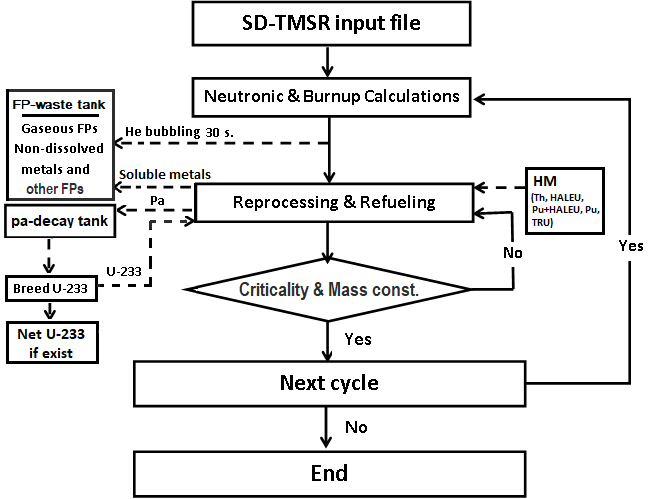
\includegraphics[width=\textwidth]{flowch1.png}
	\caption{Flow chart of the calculation procedures (implemented by SERPENT-2).}
	\label{fig:flow}
\end{figure}

As shown in Figure~\ref{fig:flow}, after launching the input file, SERPENT solves the Bateman equation using an advanced 
matrix exponential solution based on the Chebyshev Rational Approximation 
Method \cite{isotalo2016improving}. 
Then, the system extracts gaseous \gls{FPs} and other materials 
(non-dissolved metals, lanthanides, and soluble metals except Pa) with 
a suitable removal rate\footnote{The extraction rate depends on the type of 
poison and its impact on the neutron
economy.}. This is done by setting the 
flow rate of gaseous \gls{FPs} and other materials from the fuel to the 
\texttt{FP-waste tank}\footnote{An external tank used to store the gaseous 
\gls{FPs} and the other materials (non-dissolved metals, lanthanides, and 
soluble metals except protactinium).}. Specifically, Pa is removed 
from the fuel with a certain flow rate into the 
\texttt{Pa-decay tank} to decay and produce $^{233}$U \footnote{The 
$^{233}$Pa is removed and left to decay into $^{233}$U with $\tau_{1/2}$ 
$\approx$ $27$ $d$.}. The produced $^{233}$U is used as a fresh fissile fuel 
and the residual $^{233}$U (if exist) is the net production of $^{233}$U that required to start up a new SD-TMSR and achieve the transition to thorium fuel cycle. The MSR burnup 
routine provided by SERPENT-2 allows changes to the mass flow rates ($mflow$) of the 
isotopes during reactor operation \cite{aufiero2013extended}. Specifically, the SERPENT user should determine the mass flow rate ($mflow$), which is the rate by 
which elements or nuclides are transferred between materials. After that, the 
flow rates must be connected to materials with a reprocessing scheme. 
The final step is to link the reprocessing schemes to depletion histories. In 
the present work, we adjust the transfer rates of fresh fuel to maintain core 
criticality and to keep fuel salt mass constant during burnup. The continuous feed constant calculation procedures are summarized as follows:
\begin{enumerate}
	\item The simulation starts without injecting refueling materials (i.e. only removing FPs and Pa).
	\item After the first depletion calculation step, we check the total mass density of FPs and Pa in the \texttt{FP-waste tank} and \texttt{Pa-decay tank}, respectively.
	\item A simple calculation yields the amount of heavy metal that must be added during this cycle:
	\subitem 3a. \textbf{Thorium feed mechanism}: mass of injected $^{233}$U 
	$\approx$ mass of extracted Pa and mass of injected $^{232}$Th $\approx$ 
	mass of extracted FPs to maintain the total fuel mass constant.
	\subitem 3b. \textbf{Non-thorium feed mechanism}: mass of injected $^{233}$U $\approx$ mass of extracted Pa and mass of injected fuel (i.e., HALEU, Pu mixed with HALEU, reactor-grade Pu, or TRU) $\approx$ mass of extracted FPs to maintain the total fuel mass constant.
	\item Dividing this mass by time and inventory of refueling material gives the corresponding feed constant (1/s).
\end{enumerate}
In both feed mechanisms (thorium and non-thorium) we continuously added 
$^{233}$U and the mass of injected $^{233}$U is equal to the mass of extracted 
Pa ($^{233}$Pa decays to $^{233}$U after $\approx$ 27 d). To keep the total 
fuel mass almost constant, for \textbf{thorium feed mechanism}, the mass of 
injected thorium must be equal to the mass of extracted FPs and for 
\textbf{non-thorium feed mechanism}, the mass of injected fuel (i.e., HALEU, 
Pu mixed with HALEU, reactor-grade Pu, or TRU) must be equal to the mass of 
extracted FPs.

\section{Feed and extraction rates} \label{Feed-and-extraction-rates}
In the present work, two different feed mechanisms are used: (1) thorium and (2) non-thorium.
The first mechanism allows continuous feed flow of thorium from the external stockpile and 
$^{233}$U from the \texttt{Pa-decay tank}. In contrast, the second mechanism 
continuously injects external heavy metals (\gls{HALEU}, Pu mixed with \gls{HALEU}, reactor-grade Pu, \gls{TRU}) and simultaneously feeds  
all or part of produced $^{233}$U from the \texttt{Pa-decay tank}. The fission 
products (FPs) act as poisons in nuclear reactors: they negatively impact the reactivity. 
Therefore, \gls{FPs} must be extracted during reactor operation. Consider 
the \gls{MSR} extracts $dN_{e}$ amount of particular element $e$ during time $dt$, thus \cite{nuttin2005potential}:
\begin{align}
\dfrac{dN_{e}}{dt} &= N_{e}\dfrac{\varepsilon_{e}}{T_{r}}
\label{Equ:1}
\intertext{where}
dN_{e} 	&= \mbox{the amount of particular element $e$} \nonumber \\
dt   	&= \mbox{the extraction time of $dN_e$} \nonumber \\
N_{e}  	&= \mbox{total inventory of element $e$} \nonumber \\
\varepsilon_{e}	&= \mbox{the removal efficiency $\%$} \nonumber \\
T_{r}	&= \mbox{the time during which the total fuel salt is reprocessed.} \nonumber
\end{align}

Integration of equation \ref{Equ:1} gives the removal constant $\lambda_{e}$ $[s^{-1}]$ (the rate at which the material 
is removed), where $\lambda_{e}=\dfrac{{\varepsilon_{e}}}{{T}_{r}}$. The removal constant 
$\lambda_{e}$ of gaseous and other fission products is precisely calculated 
and summarized in Table~\ref{tab:table6}. The effective reprocessing time for 
the gaseous \gls{FPs} and non-dissolved metals was set to 30 s (removal 
constant $\lambda_{e}$ = $-0.0333$ $s^{-1}$), because such elements must be 
extracted promptly and continuously via a gas removal system. In contrast, 
chemical processes (i.e. fluorination and reduction) extract the soluble \gls{FPs}, lanthanides, and Pa.
Therefore, the system reprocesses a specific amount of fuel salt daily. In the 
present work, the effective extraction time for soluble \gls{FPs} is 
$\approx$10.59 days ($\lambda_{e}$ = $-1.092\times10^{-6}$ $s^{-1}$), which is 
equivalent to a chemical reprocessing rate of 5 m$^3$/d chosen by Nuttin \emph{et al.} \cite{nuttin2005potential} and Li \emph{et al.} \cite{li_optimization_2018}. The effective feed rates of 
the heavy metals (HM) are changed during reactor operation to conserve the 
total fuel mass and criticality. The effective feed rates for Th/$^{233}$U, reactor-grade Pu, and TRU cases are listed in Table A.1, A.2, and A.3 in \ref{Appendix}.


\begin{table}[ht!]
	\centering
	\caption{The reprocessing table \cite{ashraf2019whole_core,ashraf2019Preliminary}.} 
	\vspace{1ex}
	\begin{tabularx}{\textwidth}{|p{2.3cm}|p{4cm}|p{2.2cm}|p{1.9cm}|}
			\hline
			\textbf{Reprocessing group}  & \textbf{Element} & \textbf{Reprocessing time} & \textbf{Removal constant} $\lambda_{e}$ $[s^{-1}]$ \\
			\hline
			\raggedright Gaseous \gls{FPs} and non-dissolved metals  &  H, He, N, O, Ne, Ar, Kr, Nb, Mo, Tc, Ru, Rh, Pd, Ag, Sb, Te, Xe, Lu, Hf, Ta, W, Re, Os, Ir, Pt, Au, and Rn.		&	\raggedright 30 s	&  -3.333E-02 \\
			\hline
			\raggedright Lanthanides and other soluble \gls{FPs}     & 
			Zn, Ga, Ge, As, Se, Br, Rb, Sr, Y, Zr, Cd, In, Sn, I, Cs, Ba, La, Ce, Pr, Nd, Pm, Sm, Eu, Gd, Tb, Dy, Ho, Er, Tm, and Yb. & \raggedright 10.59 d (5 m$^3$/d) &  -1.092E-06 \\
			\hline
			Protactinium   & Pa  & \raggedright 10.59 d (5 m$^3$/d)  &  -1.092E-06 \\
			\hline
	\end{tabularx}
	\label{tab:table6}
\end{table}
\FloatBarrier
\section{Results and discussion} \label{Results-and-discussion}
The molar fraction of the heavy metal (HM) 
in the initial fuel was kept constant and equal to 12.5 mole\% for all cases (see Table~\ref{tab:table4}). 
Additionally, the initial fissile material fraction was increased for the five fuel 
salt compositions until the SD-TMSR reactor was sufficiently critical at 
the Beginning Of Life (BOL).
\subsection{Thorium feed mechanism}
The thorium feed mechanism continuously feeds thorium from the external stockpile and 
$^{233}$U from the \texttt{Pa-decay tank}.
Figure~\ref{fig:keff1} illustrates the effective multiplication factor 
dynamics during reactor operation for the thorium feed mechanism. As shown in 
Figure~\ref{fig:keff1}, the effective multiplication factor ($k_{eff}$) 
decreases sharply during the first 25 \gls{EFPY} of reactor operation for the first 
four cases. $k_{eff}$ decreases as a result of depletion of the initial 
fissile materials and production of poisonous fission products (FPs). The amount of $^{233}$U generated in 
the SD-TMSR is not enough to maintain the reactor criticality and 
counteract parasitic neutron absorption. Thus, the 
reactor becomes subcritical relatively quickly for alternative startup 
compositions, for example, $\approx$ $4$ years in the \gls{TRU} case and $\approx$ $12$ 
years in the reactor-grade Pu case. For U-233 case, 
the continuous feed flow of thorium and $^{233}$U from the \texttt{Pa-decay tank} helps to operate the 
SD-TMSR for a full lifetime (60 year) (Figure~\ref{fig:keff1}, U-233 case).

Notably, the molar fractions of \gls{HALEU} and reactor-grade Pu in the initial fuel composition were increased
more. Consequently, the initial $k_{eff}$ for these cases increased (Figure~\ref{fig:keff1} (HALEU and reactor-grade Pu cases)).
For the HALEU fuel salt, the amount of $^{233}$U generated in the SD-TMSR after a few years is insufficient to counteract the absorption of the (non-fissile) $^{238}$U added at start-up after much of the original $^{235}$U is depleted. Consequently, the core becomes subcritical after $\approx$ $6$ years of operation.

For Pu+HALEU case, K${_eff}$ firstly increases during the first $\approx$ $3$ EFPY and after that decreases. This is due to the conversion of $^{238}$U from HALEU into fissile plutonium, which often produces the majority of the fission power until the transition to Th/$^{233}$U fuel cycle. Figure~\ref{fig:diffPuAll811} shows the variation of fissile plutonium isotopes ($^{239}$Pu , $^{241}$Pu, and $^{243}$Pu) during reactor operation. For TRU and reactor-grade Pu, the fissile plutonium isotopes are depleted, during operating (the fissile material is dominated by Pu in these cases). For HALEU case, the fissile material is dominated by $^{235}$U, however, $^{238}$U is converted into fissile plutonium. Therefore, the mass of fissile plutonium increases during operating but its value still relatively low. For Pu+HALEU case, the mass of the fissile plutonium isotopes increases within the first $\approx$ 3 EFPY and then decreases. The reactivity from the produced Pu is much greater than the depletion of the initial reactivity (due to the depletion of initial fissile isotopes), consequently, K${_eff}$ increases during the first $\approx$ 3 years and then decreases; the amount of $^{233}$U generated in the Pu+HALEU case is insufficient to maintain the reactor criticality and counteract neutron absorption in non-fissile isotopes.

Figure~\ref{fig:keff1} shows that the decrease in K${_eff}$ for reactor-grade Pu case occurs at a much later operating time than for other cases, this is because of the neutron spectrum in the reactor-grade Pu initial core is hardened; more $^{232}$Th is being converted to $^{233}$U. Nevertheless, this amount of the $^{233}$U is not enough to counteract the neutron absorption in the non-fissile Pu isotopes after much of the $^{239}$Pu and $^{241}$Pu is depleted \cite{betzler2016modeling}.

\begin{figure}
	\centering
	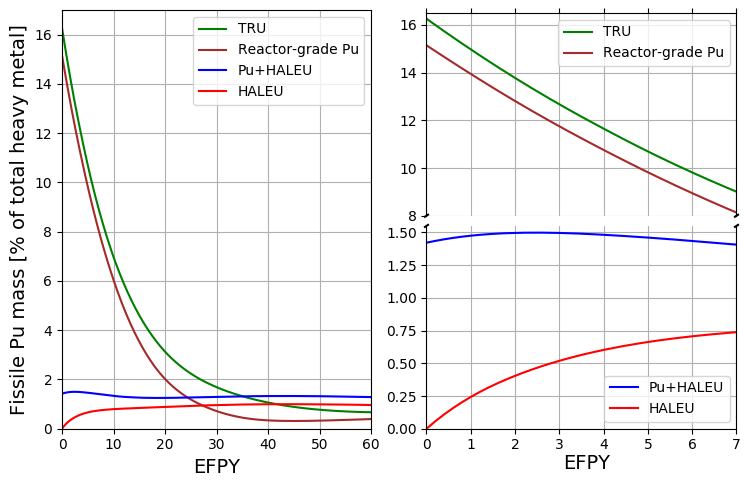
\includegraphics[width=\textwidth]{diffPuAll811.png}
		\vspace{-0.5in}
	\caption{The variation of relative mass of fissile Pu ($^{239}$Pu , $^{241}$Pu, and $^{243}$Pu) during reactor operation.} 
	\label{fig:diffPuAll811}
\end{figure}

\begin{figure}
	\centering
	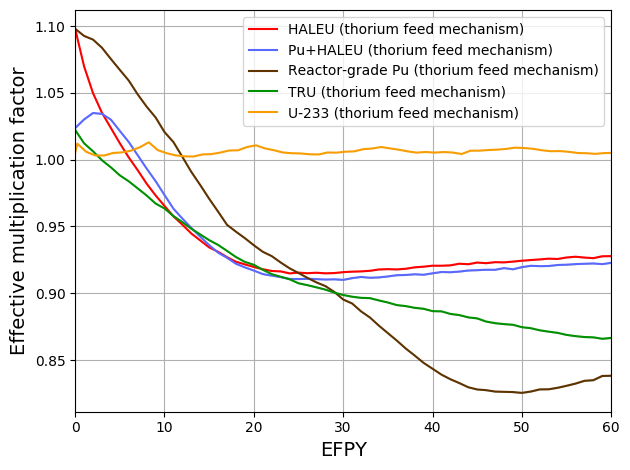
\includegraphics[width=\textwidth]{keff1.png}
	\vspace{-0.5in}
	\caption{The change of the effective multiplication factor during 60 \gls{EFPY} of reactor operation for thorium feed mechanism (confidence interval $\pm\sigma$ is shaded).} 
	\label{fig:keff1}
\end{figure}

\subsection{Non-thorium feed mechanism}
The non-thorium feed mechanism continuously feeds 
$^{233}$U from the \texttt{Pa-decay tank} and external heavy metals (\gls{HALEU}, Pu mixed with \gls{HALEU}, reactor-grade Pu, \gls{TRU}).
Under the non-thorium feed mechanism, only four different initial fissile materials are studied: \gls{HALEU}, Pu mixed with \gls{HALEU}, reactor-grade Pu, and \gls{TRU}. The continuous feed of $^{233}$U 
without $^{232}$Th will lead to a supercritical reactor, thus the $^{233}$U case 
is excluded from the non-thorium feed mechanism study.
Figure~\ref{fig:keff2} shows the change of the effective multiplication factor 
during 60 \gls{EFPY} of reactor operation for the non-thorium feed mechanism. Both the reactor-grade Pu and TRU cases 
show promising results relative to the other two cases (HALEU and Pu+HALEU) (see Figure~\ref{fig:keff2}). 
\begin{figure}
	\centering
	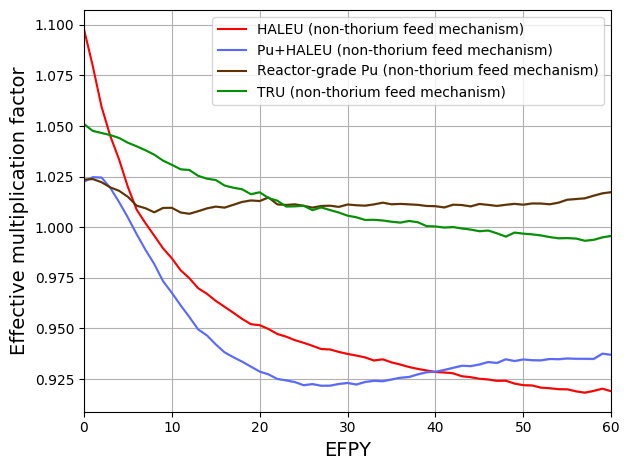
\includegraphics[width=\textwidth]{keff2.png}
			\vspace{-0.5in}
	\caption{The change of the effective multiplication factor during 60 
	\gls{EFPY} of reactor operation for non-thorium feed mechanism (confidence 
	interval $\pm\sigma$ is shaded).} 
	\label{fig:keff2}
\end{figure}
For the reactor-grade Pu case, the amount of $^{233}$U generated in the SD-TMSR, in addition to the external feed flow of Pu, is sufficient to maintain the reactor criticality and counteract the neutron absorption in the initial non-fissile isotopes and FPs. 
For the \gls{TRU} fuel salt, the amount of 
$^{233}$U and the external feed flow of TRU is barely enough to operate the 
reactor for a long period of time ($\approx$ $40$ years) without any 
external feed of $^{233}$U ($^{233}$U used only from the \texttt{Pa-decay tank}). Nevertheless, $k_{eff}$ decreases with the burnup 
because of the \glspl{MA}\footnote{In the present work, the minor actinides 
(MA) include Np, Am, and Cm.} accumulating in the core as a result of 
continuous TRU feed. As shown in Figure~\ref{fig:keff2}, the HALEU and Pu+HALEU 
fuel are less attractive for the non-thorium feed mechanism. The continuous HALEU 
feed increases the amount of fertile $^{238}$U and consequently, reduces the 
feasibility of such fissile materials. According to the $k_{eff}$ 
results, reactor-grade Pu and TRU are the only alternative fissile materials that  
can be used to startup and maintain operation of the SD-TMSR.

\subsection{Reactor-grade Pu, TRU, and $^{233}$U initial fuel}
In this section, the simulation of the SD-TMSR with reactor-grade Pu and TRU 
fissile materials is discussed. Additionally, the previously studied $^{233}$U 
case is listed for comparison \cite{ashraf2019whole_core}. 
Figure~\ref{fig:refillCCC} demonstrates the dynamics of the heavy metal refill 
rate during 60 \gls{EFPY} of the SD-TMSR operation. The heavy metal refill 
rate was adjusted to maintain criticality and the total fuel mass 
almost constant\footnote{The variation of the total fuel mass is less than 
$0.1\%$} during reactor operation. In the $^{233}$U case, the mean values of 
$^{233}$U and $^{232}$Th refill rate are $1.77$ and $2.21$ $kg/d$, 
respectively. Similarly, in the reactor-grade Pu case, the mean values of 
$^{233}$U and Pu refill rate are $0.75$ and $2.75$ $kg/d$, respectively. For  
the TRU case, the mean values of $^{233}$U and TRU refill rate are $0.90$ and 
$2.0$ $kg/d$, respectively.
\begin{figure}
	\centering
	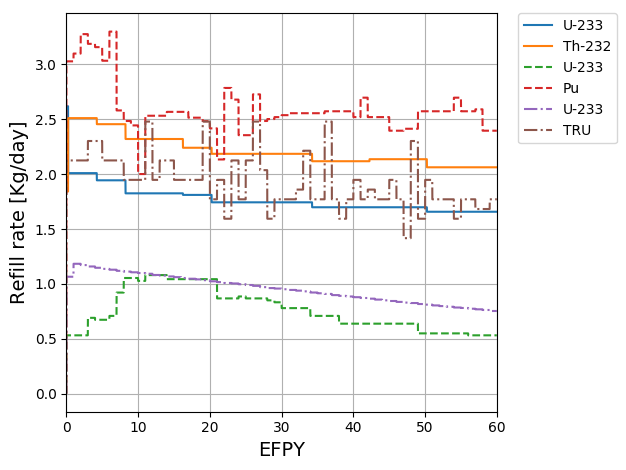
\includegraphics[width=\textwidth]{refillCCC.png}
			\vspace{-0.5in}
	\caption{Dynamics of heavy metal refill rate during 60 \gls{EFPY} of 
		reactor operation. Solid lines for the $^{233}$U case, dashed lines for the
		reactor-grade Pu case, and dotted lines for the TRU case.}
	\label{fig:refillCCC}
\end{figure}

Figures~\ref{fig:inventoryCCCC} and~\ref{fig:inventoryPu_TRUCCC} demonstrate 
the evolution of important nuclide inventories for the $^{233}$U, Pu, and TRU cases 
respectively. For the $^{233}$U case (Figure~\ref{fig:inventoryCCCC}), the mass of Pa in the fuel salt is almost constant and reaches 
$17.8$  $kg$ at the end of the operation time. 
Additionally, the mass of minor actinides (MA) and Pu increases with time. The level of Pu in the fuel salt correlates with the mass of the MA; however, MA need more time to reach equilibrium than Pu. Uranium inventory increases during 
operation and reaches equilibrium after $\approx$ $27$ years. Figure~\ref{fig:inventoryCCCC} shows that refueling the core with thorium helps 
maintain an almost constant inventory throughout the full operation time. 
For the Pu and TRU cases (Figure~\ref{fig:inventoryPu_TRUCCC}), the Pa extraction time was selected to be 30 s 
to avoid poisoning the core. Figure~\ref{fig:inventoryPu_TRUCCC} shows that the mass of Pa in the fuel salt 
is relatively low when compared to Pa mass in the $^{233}$U case (Figure~\ref{fig:inventoryCCCC}). Major 
elements for all three cases reach the equilibrium state after $\approx$ $30$ 
years (see Figure~\ref{fig:inventoryCCCC} and~\ref{fig:inventoryPu_TRUCCC}).
\begin{figure}
	\centering
	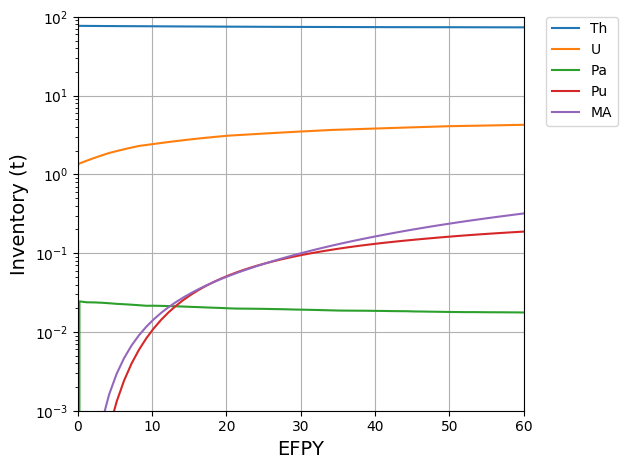
\includegraphics[width=\textwidth]{inventoryCCCC.png}
	\vspace{-0.4in}
	\caption{Evolution of important nuclide inventories for $^{233}$U 
		startup fuel (MA involves Np, Am, Cm) \cite{ashraf2019whole_core}.}
	\label{fig:inventoryCCCC}
\end{figure}
\begin{figure}
	\centering
	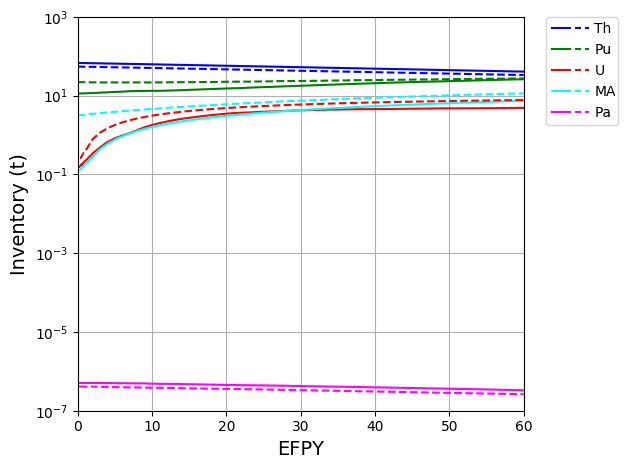
\includegraphics[width=\textwidth]{inventoryPu_TRUCCC.png}
	\vspace{-0.5in}
	\caption{Evolution of important nuclide inventories for the 
		reactor-grade Pu case (solid lines) and for the TRU case (dashed lines).}
	\label{fig:inventoryPu_TRUCCC}
\end{figure}

Figure~\ref{fig:Th232CC} illustrates the variation of thorium inventory in the 
fuel salt for the $^{233}$U, reactor-grade Pu, and TRU cases. The thorium inventory 
decreases in the $^{233}$U case by only $3.2$\% at the End Of Life (EOL) when the thorium 
feed mechanism is applied. 
In contrast, thorium total mass decreases significantly in the Pu and TRU cases when the non-thorium 
feed mechanism is applied. Thus, thorium mass decreases by $39.21$\% and 
$37.96$\% for the reactor-grade Pu and TRU cases, respectively.
\begin{figure}
	\centering
	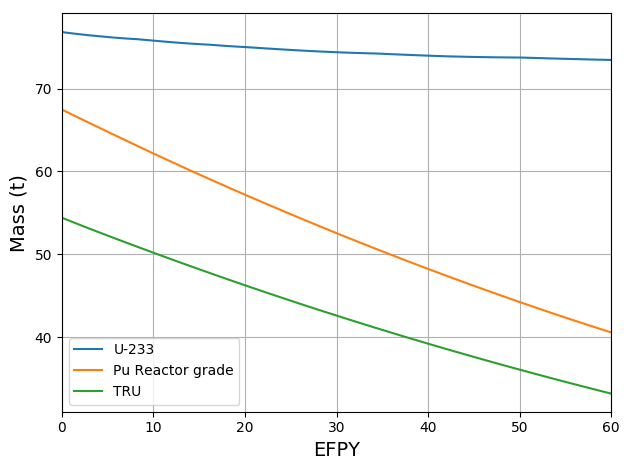
\includegraphics[width=\textwidth]{Th232CC.png}
	\caption{Mass variation of all thorium isotopes in the fuel salt for the $^{233}$U, reactor-grade Pu, and TRU cases.}
	\label{fig:Th232CC}
\end{figure}

Figure~\ref{fig:U233CC} demonstrates the mass of $^{233}$U in the fuel salt for the $^{233}$U, reactor-grade Pu, and TRU cases. For $^{233}$U case, the mass of $^{233}$U increases with operating time and reaches $\approx$ $1.7$ $t$ at the EOL. For reactor-grade Pu and TRU cases, the mass of $^{233}$U firstly, increases and after $\approx$ $35$ and $45$ years for Pu and TRU cases, respectively, decreases. The neutron spectrum shift during operating affects the inventory of $^{233}$U in the fuel salt. Hard neutron spectrum converts more $^{233}$U from $^{232}$Th. For the reactor-grade Pu and TRU cases, during operating, the fissile Pu is depleted and the $^{233}$U becomes the major fissile isotope; the neutron spectrum softens (low conversation of $^{233}$U from $^{232}$Th). However, for $^{233}$U case, the neutron spectrum is hardened at EOL due to the accumulation of Pu isotopes.

\begin{figure}
	\centering
	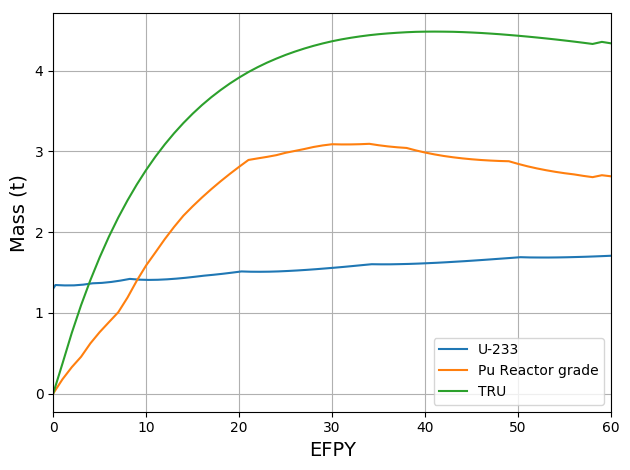
\includegraphics[width=\textwidth]{U233CC.png}
	\caption{Mass of $^{233}$U in the fuel salt for the $^{233}$U, reactor-grade Pu, and TRU cases.}
	\label{fig:U233CC}
\end{figure}

In the non-thorium feed mechanism, the SD-TMSR is continuously refueled by heavy metals (Pu and TRU) for 
criticality, which increases the Pu mole concentration (\%) in the molten salt. 
The Pu solubility in FLiBe is 
$\approx$ $4.0$ \% \cite{ignatiev2012progress,sood1975plutonium}. 
Figure~\ref{fig:PusolubilityCC} represents the Pu mole concentration variation in the fuel salt 
for the $^{233}$U, reactor-grade Pu, and TRU cases, respectively. In the $^{233}$U and reactor-grade Pu cases, the Pu mole concentration increases 
slightly but still below its solubility limit. On the other hand, the Pu 
mole concentration in the molten salt loaded by TRU increases during operation and 
reaches the Pu solubility limit after $\approx$ $40$ years. This issue may 
be solved by increasing the reactor operation temperature or reducing the 
HM initial inventory \cite{zou2018transition}. Notably, for TRU case, the time achieving Pu solubility limit is shorter than that for reactor-grade Pu case. The reason for this is the relatively high concentration of Pu in the initial heavy metal for the TRU-started SD-TMSR ($\approx$ $29.26$ \% compared with $14.31$ \% for Pu-started SD-TMSR, see Table~\ref{tab:table5}).

\begin{figure}
	\centering
	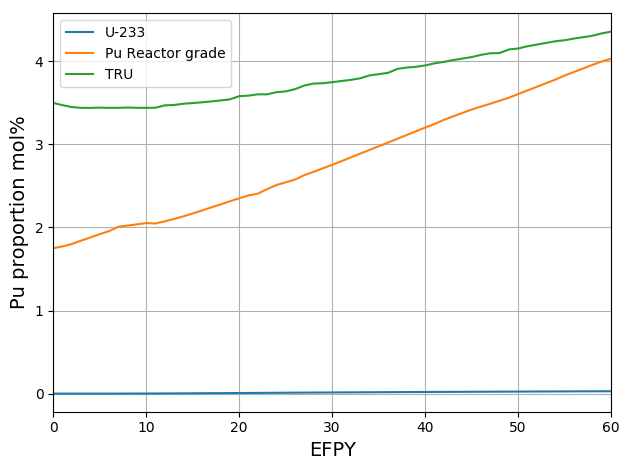
\includegraphics[width=\textwidth]{PusolubilityCC.png}
	\caption{The Pu mole concentration in the fuel salt for the $^{233}$U, reactor-grade Pu, and TRU cases.}
	\label{fig:PusolubilityCC}
\end{figure}
\FloatBarrier

Figure~\ref{fig:NetCC} demonstrates the net production of $^{233}$U during 
reactor operation for the $^{233}$U, reactor-grade Pu, and TRU cases, respectively. For the TRU case, the net production of $^{233}$U is almost 
zero. 
Although all produced $^{233}$U is used to refuel the core, the reactor is subcritical after $40$ years of operation (see Figure~\ref{fig:keff2}).
In the $^{233}$U and reactor-grade Pu cases, the net production of 
$^{233}$U increases with burnup and reaches about $1.77$ $t$ and $10$ $t$ at EOL, respectively. Figure~\ref{fig:NetCC} shows that for the $^{233}$U 
case the net production of $^{233}$U during the first 455 days is negative; 
about $175.28$ $kg$ of $^{233}$U must be added during this period. 
As shown in Figure~\ref{fig:NetCC}, for the $^{233}$U case, after 26 years the net production of $^{233}$U reaches 
$1.3$ $t$; this is sufficient to start up another SD-TMSR (see Table~\ref{tab:table5}). Similarly, 
one can see that the same amount of $^{233}$U ($1.3$ $t$) can be achieved 
after $\approx$ $4.5$ years if we apply the non-thorium feed mechanism on 
the SD-TMSR that was initially loaded by reactor-grade Pu alternative to 
$^{233}$U. For nonproliferation reasons, $^{233}$U could be diluted with $^{238}$U which makes it impossible to use for nuclear weapons.
  
In conclusion, the thorium fuel cycle transition can be achieved by selecting the 
proper feed mechanism and initial fissile material. 
Specifically, applying the non-thorium feed mechanism on 
the SD-TMSR loaded by reactor-grade Pu allows the 
transition to the thorium fuel cycle after $\approx$ 
$4.5$ years. Additionally, applying the thorium feed mechanism on 
the SD-TMSR loaded by $^{233}$U allows the 
transition to the thorium fuel cycle after $\approx$ $26$ years of operation. 
The comparison between the two feed mechanisms with various initial fuel types 
is listed in Table~\ref{tab:comp_feeds}. 

\begin{figure}
	\centering
	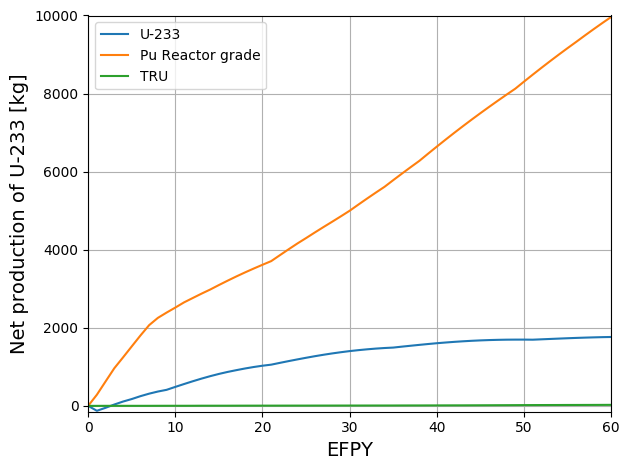
\includegraphics[width=\textwidth]{NetCC.png}
	\caption{Net production of $^{233}$U with burnup (60 \gls{EFPY}) for the $^{233}$U, reactor-grade Pu, and TRU cases.}
	\label{fig:NetCC}
\end{figure}

\begin{table}  [!h]
	\begin{minipage}{\linewidth}
		\renewcommand\footnoterule{}
		\renewcommand{\thefootnote}{\alph{footnote}}
		\caption{Comparison between the two feed mechanisms for the five different 
			types of initial fuel.}
		\label{tab:comp_feeds}
		\vspace{0.1in}
		\begin{tabularx}{\textwidth}{p{0.22\textwidth} X p{0.18\textwidth} 
				p{0.14\textwidth} X X 
			}  %{\textwidth}
			\hline
			Feed mechanism & \gls{HALEU} (19.79\%) & Pu+\gls{HALEU} (19.79wt.\%) &  
			reactor-grade Pu & \gls{TRU}& $^{233}$U \\
			\hline
			Thorium feed\\ mechanism&\xmark&\xmark&\xmark&\xmark& \cmark \\
			Non-thorium feed\\ mechanism &\xmark&\xmark&\cmark\footnotemark[1] 
			&\cmark\footnotemark[2] & \xmark\footnotemark[3] \\
			\hline
		\end{tabularx}
		\vspace{-1.5ex}%
		\footnotetext[1]{Positive $^{233}$U net production and critical 
			configuration for 60 years of operation.}
		\footnotetext[2]{Zero $^{233}$U net production and critical 
			configuration for 40 years of operation.}		
		\footnotetext[3]{Too large and increasing $k_{eff}$ during 
			lifetime.}		
	\end{minipage}
\end{table}
\FloatBarrier

\subsection{Neutron spectrum}
Figure~\ref{fig:spectrumFLUX110vC} represents the neutron flux per unit 
lethargy for a full-core SD-TMSR model in the energy range from 10$^{-8}$ to 
10 MeV for the $^{233}$U, reactor-grade Pu, and TRU cases at BOL and EOL. In 
the $^{233}$U case, at the EOL, the neutron spectrum is harder than at BOL due 
to the accumulation of Pu and other strong thermal neutron absorbers in the 
fuel salt. For the reactor-grade Pu and TRU cases, during reactor operation, 
the fissile Pu is depleted and the $^{233}$U becomes the major fissile isotope 
(see Figure~\ref{fig:U233CC}); the neutron spectrum softens and becomes 
similar to the initial thermal spectrum of a $^{233}$U fueled SD-TMSR.
The neutron spectrum of TRU case at BOL is softer than $^{233}$U case because $^{232}$Th inventory is much lower for the TRU case: $54.4$ $t$ instead of $76.9$ $t$ for the $^{233}$U. $^{232}$Th has a very high absorption cross section in the thermal region ($\approx10^2 $b). Moreover, $^{232}$Th has resonance region between $10^{-5}$ and $10^{-3}$ which justify relatively low energy of neutrons for the TRU case in this energy range (see Figure~\ref{fig:spectrumFLUX110vC}).
 \begin{figure}
 	\centering
 	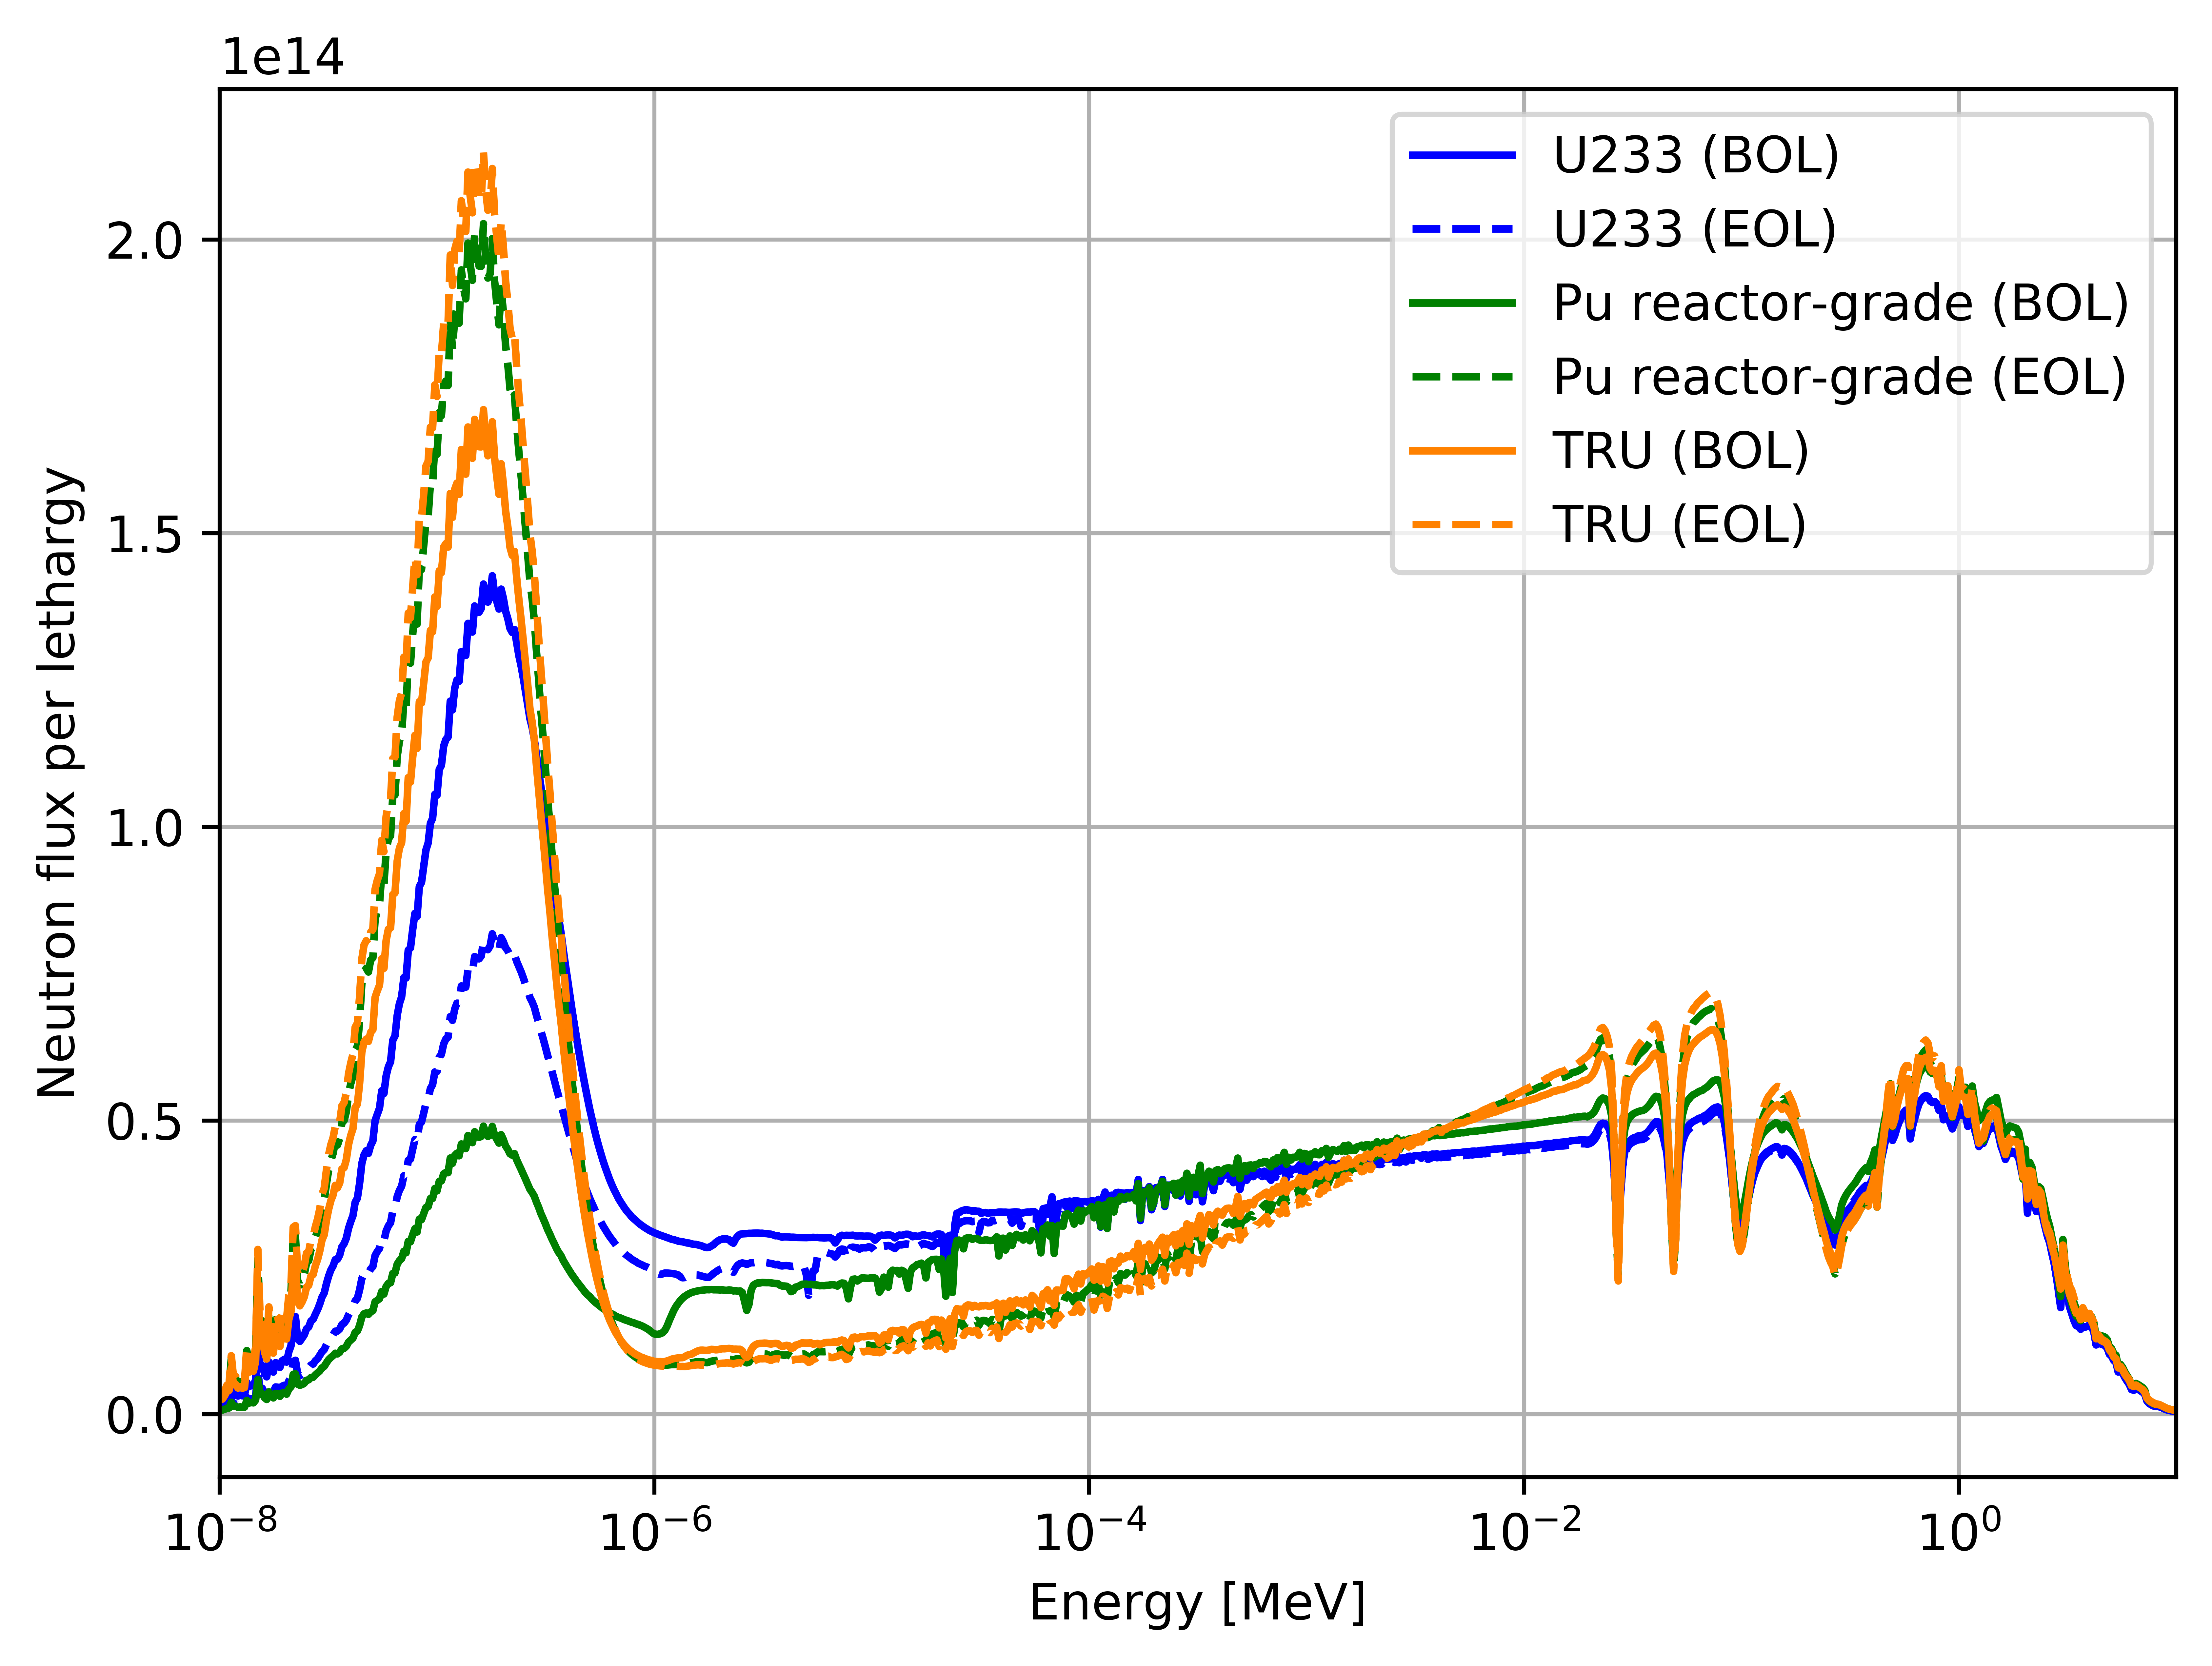
\includegraphics[width=1.01\textwidth]{spectrumFLUX110vC.png}
 			\vspace{-0.4in}
 	\caption{The neutron flux energy spectrum at BOL (solid lines) and EOL (dashed lines) for 3 different initial 
 		fuel salt compositions (for all cases, the neutron flux
 		confidence intervals $\pm\sigma$ at BOL and EOL are $<1.0139$\% and $<0.6274$\%, respectively).}
 	\label{fig:spectrumFLUX110vC}
\end{figure}

\subsection{Neutron flux}
Figures~\ref{fig:fast_flux} and \ref{fig:thermal_flux} show the radial 
distribution of fast (energy range between 0.625 eV and 20 MeV) and thermal 
(energy range between 10$^{-5}$ eV and 0.625 eV) neutron flux for three 
different initial fissile materials in the fuel salt ($^{233}$U, reactor-grade 
Pu, TRU) at startup and at equilibrium (after $\approx 30$ years of 
operation). Actinides' evolution and poisonous fission product accumulation 
for various initial fissile compositions demonstrates the different effects on 
the SD-TMSR neutronics performance. For the $^{233}$U case, the thermal 
neutron flux is suppressed at equilibrium because fissile $^{233}$U in the 
core is being substituted with heavier fissile actinides: $^{235}$U, 
$^{239}$Pu, and $^{241}$Pu. This agrees with results in literature 
\cite{rykhlevskii2019modeling, ashraf2019whole_core}.
\begin{figure}[htp!] % replace 't' with 'b' to force it to \centering
	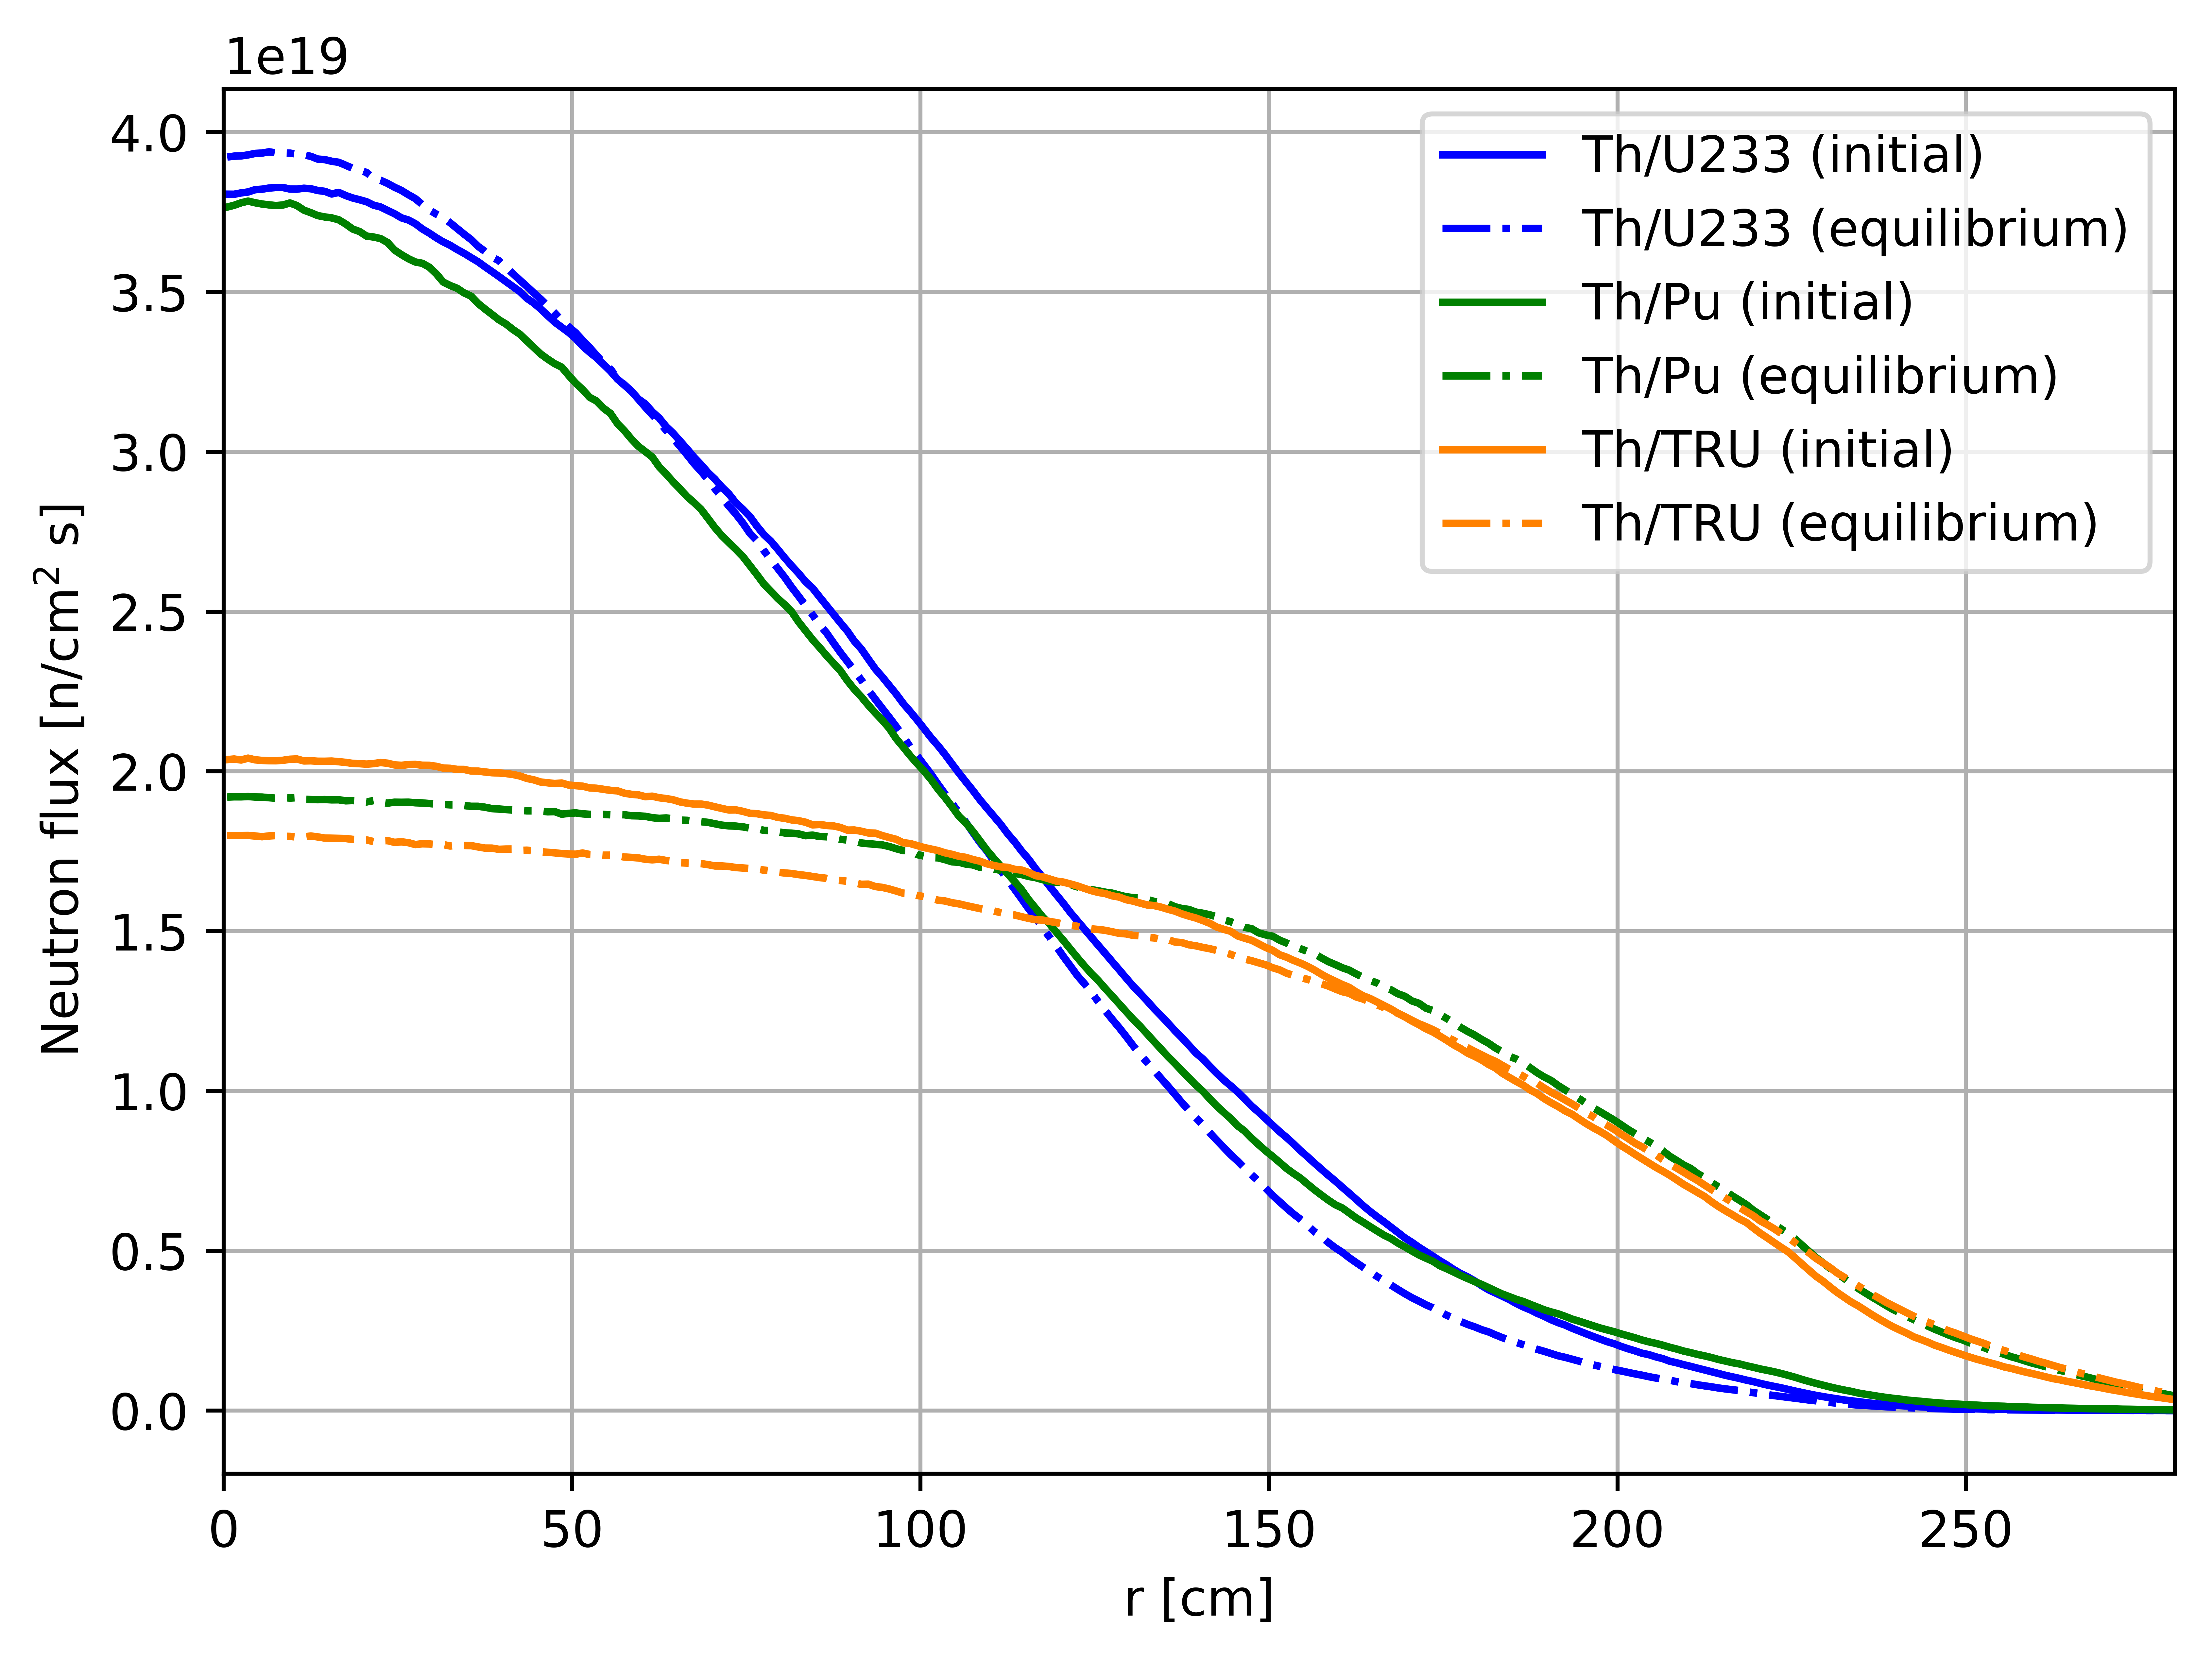
\includegraphics[width=\textwidth]{radial_fast_flux_init_vs_eq.png} 
	\caption{Radial fast neutron flux distribution for 3 different initial 
		fuel salt compositions at startup and equilibrium (the fast flux 
		confidence interval $\pm\sigma<2.5$\% for all cases).}
	\label{fig:fast_flux}
\end{figure}

Opposite behavior is observed for the reactor-grade Pu and TRU cases. For  
these cases, the thermal neutron flux increases during operation while fast 
neutron flux decreases. Fissile Pu nuclides (generate relatively hard 
spectrum) from initial fuel salt composition are gradually substituted with  
$^{233}$U (generates relatively soft spectrum), produced from fertile 
$^{232}$Th. During reactor operation, $^{233}$U becomes the primary fissile 
isotope, which softening the neutron spectrum of the reactor. 
\begin{figure}[htp!] % replace 't' with 'b' to force it to \centering
	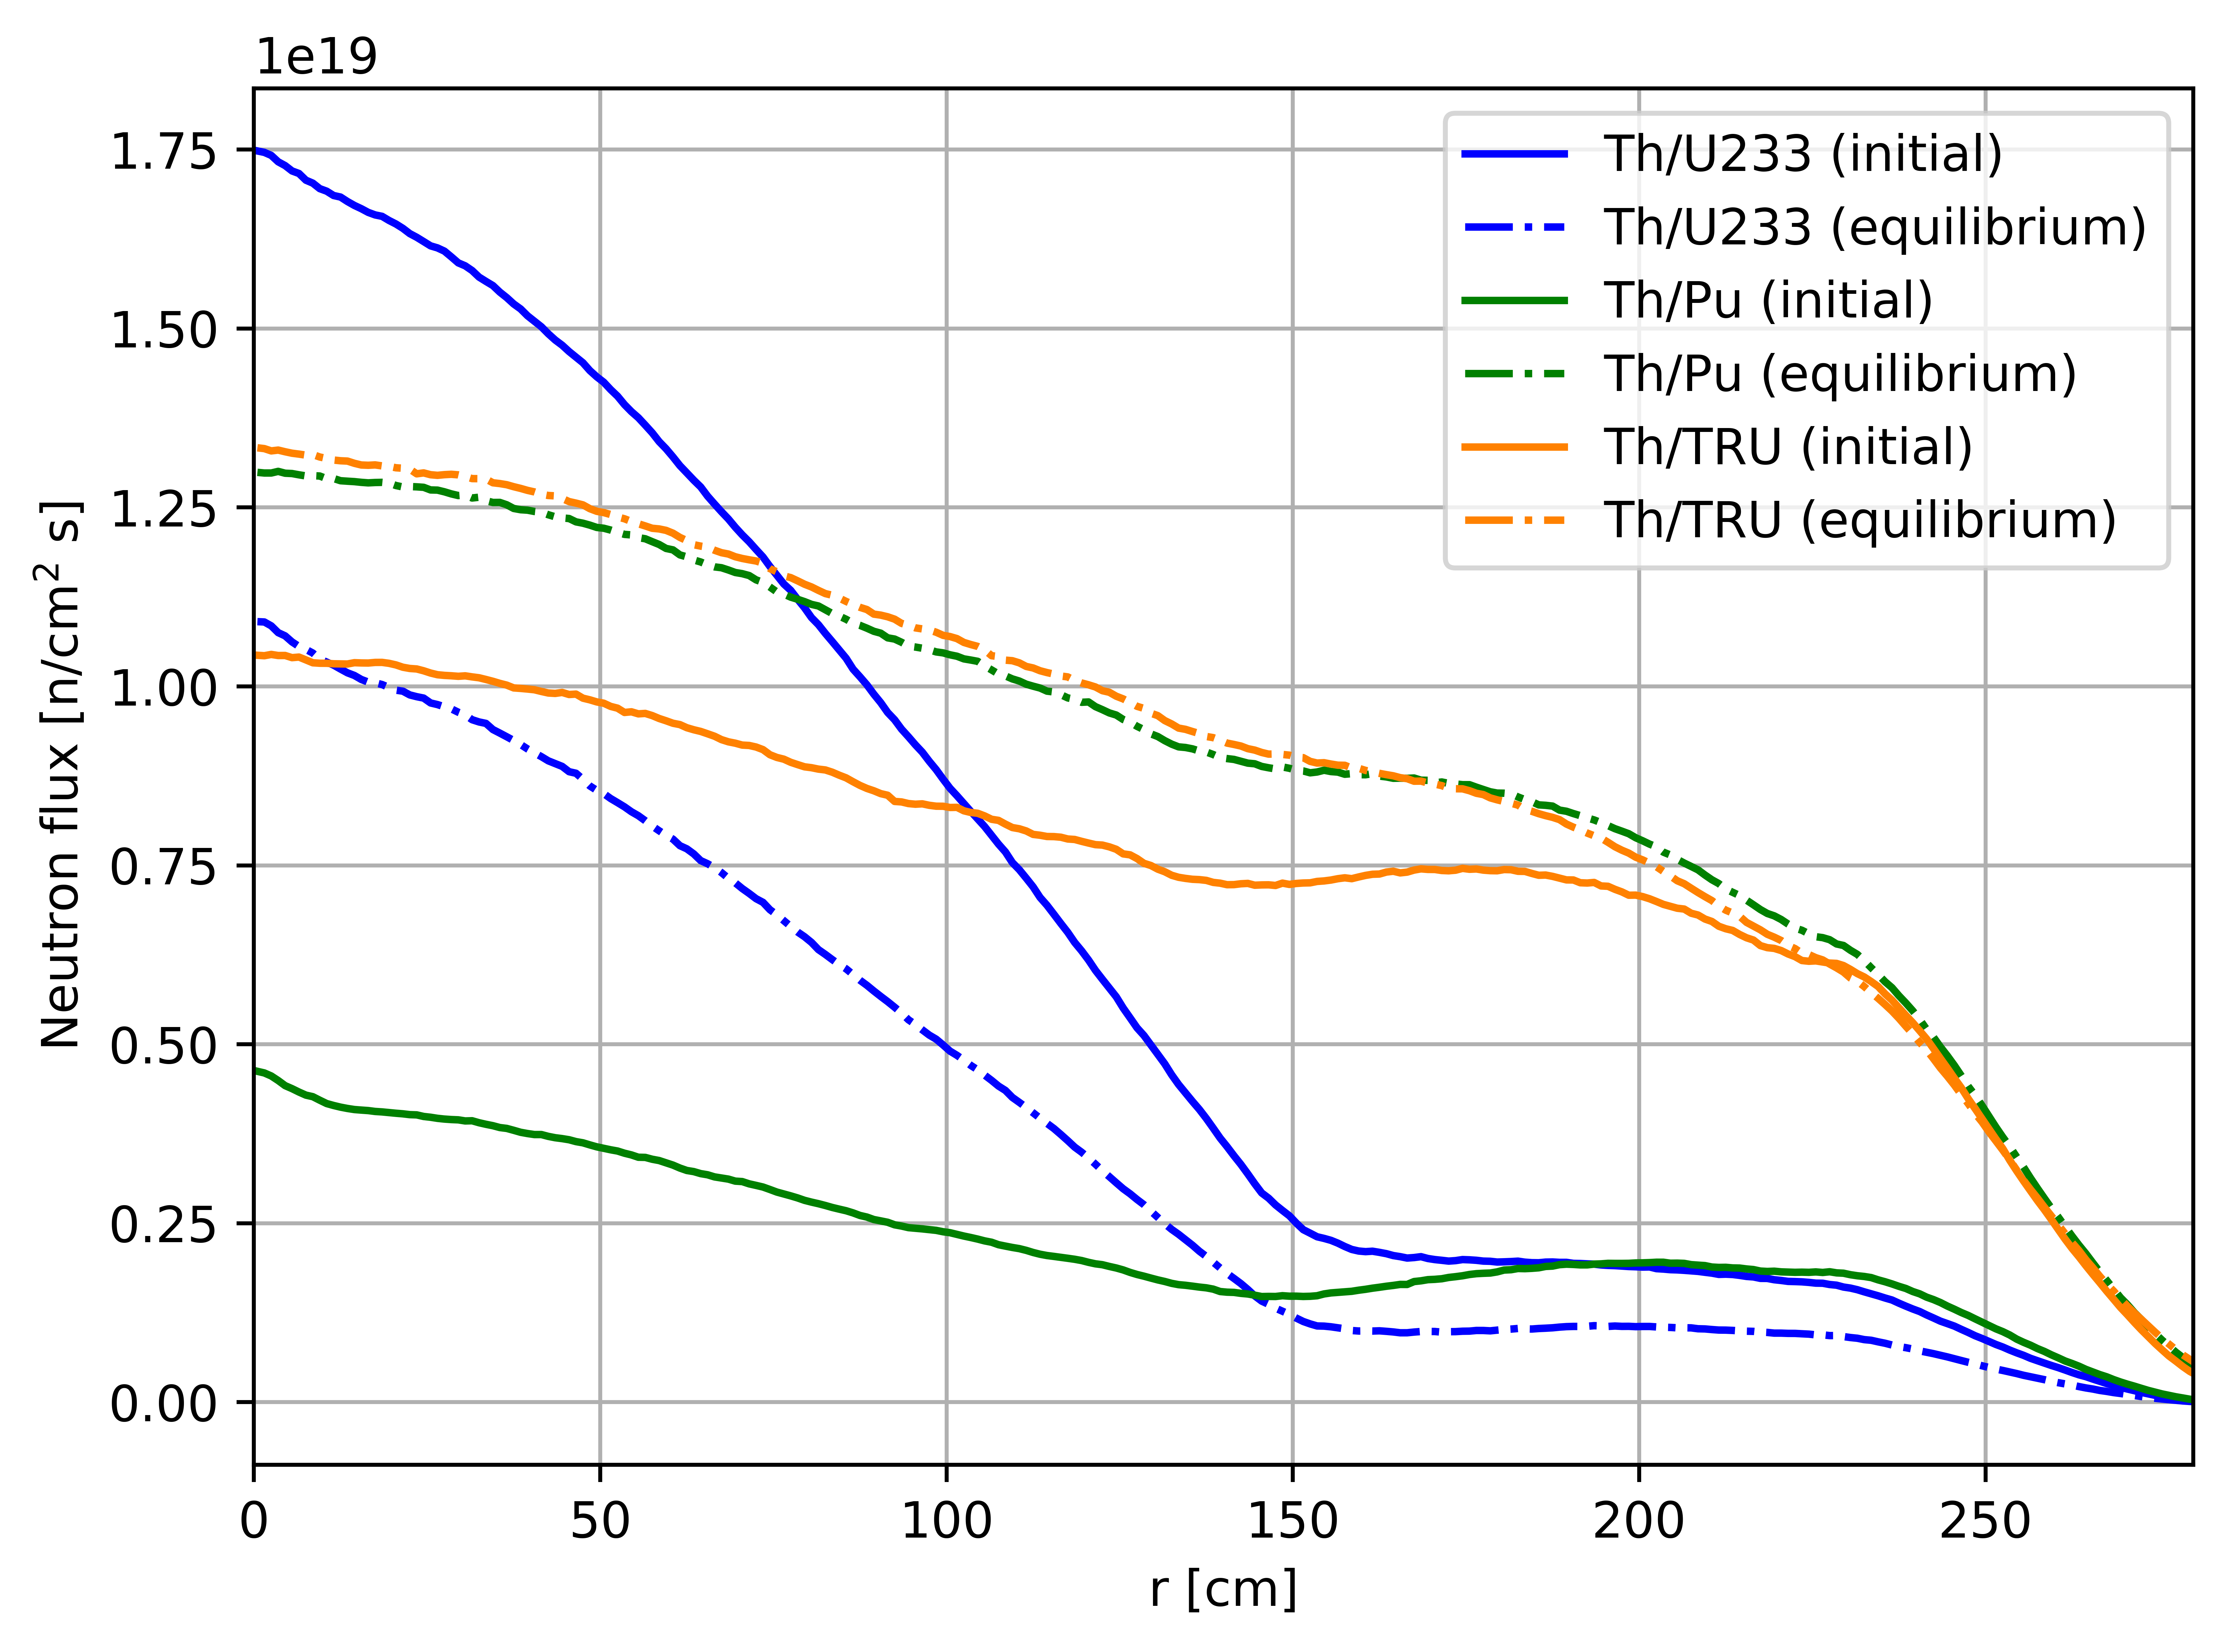
\includegraphics[width=\textwidth]{radial_thermal_flux_init_vs_eq.png} 
	\caption{Radial thermal neutron flux distribution for 3 different initial 
		fuel salt compositions at startup and equilibrium (the thermal flux 
		confidence interval $\pm\sigma<1.6$\% for all cases).}
	\label{fig:thermal_flux}
\end{figure}

More changes in thermal neutron flux shape and magnitude for the 
$^{233}$U case are observed in the inner core zone ($R\lesssim150$) than 
in the outer core zone. In contrast, for the reactor-grade Pu and TRU cases, 
significant changes are observed for thermal neutron flux in the outer core 
zone and reflector. Additionally, Figure~\ref{fig:thermal_flux} shows 
relatively large changes in thermal flux leakage from the core for the Pu and 
TRU cases. The SD-TMSR core design was optimized for $^{233}$U  
\cite{li_optimization_2018}, thus, the core geometry (e.g., channels lattice 
pitch) must be re-optimized for another type of fuel to obtain better 
neutronics performance.

\subsection{Temperature coefficient of reactivity}
The temperature coefficient of reactivity quantifies reactivity changes due to 
temperature increase in the core and is calculated in this work as follows:
\begin{align}
\alpha &= \frac{k_{eff}(T_{i+1}) - k_{eff}(T_i)}{k_{eff}(T_{i+1}) 
	k_{eff}(T_{i}) (T_{i+1} - T_i)}
\intertext{where}
k_{eff} &= \mbox{effective multiplication factor} \nonumber \\
T_i &= \mbox{fuel salt temperature in (900 K, 1000 K).} \nonumber
\end{align}

Table~\ref{tab:tcoe} summarizes temperature coefficients calculated for three 
different initial fissile loads at startup and at equilibrium. By propagating 
the $k_{eff}$ statistical error provided by SERPENT-2, uncertainty for each 
temperature coefficient is calculated using the following formula:
\begin{align}
\delta\alpha &= \abs{\frac{1}{T_{i+1} - T_i}} \sqrt{\frac{\delta 
		k_{eff}^2(T_{i+1})}{k_{eff}^4(T_{i+1})}  
	+ \frac{\delta k_{eff}^2(T_i)}{k_{eff}^4(T_i)}}
\intertext{where}
\delta k_{eff} &= \mbox{statistical error for $k_{eff}$ from SERPENT-2 
output.} 
\nonumber
\end{align}

Other sources of uncertainty are neglected, such as cross section measurement 
error and approximations inherent in the density dependence on temperature. 

When the fuel salt temperature increases, the density of the salt decreases, 
but at the same time, the total volume of fuel salt in the 
core remains constant because it
is bounded by the vessel. When the graphite 
temperature increases, the density of
graphite decreases, creating additional 
space for the salt. The cross section temperatures for the fuel and moderator 
were changed from 900 to 1000 K to determine the temperature coefficients. 
This work considered five different cases:
\begin{enumerate}
	\item Fuel salt temperature (Doppler Effect) rising from 900 to 1000 K 	
	(first row in Table~\ref{tab:tcoe}).
	\item Fuel salt density decreasing from 3.3 to 3.233 g/cm$^3$ 
	(density change caused by temperature increase from	900 to 1000 K).
	\item Total fuel salt temperature (Doppler+density) rising from 900 to 
	1000 K.	
	\item Graphite temperature (Doppler Effect) rising from 900 to 1000 K.
	\item Whole reactor temperature rising from 900 K to 1000 K.
\end{enumerate}

In the first case, the fuel temperature change only impacts cross section 
temperature. In the second case, changes in the fuel temperature only impact 
density, and the third case takes into account both effects. The geometry for 
these three cases is unchanged because the fuel is a liquid. However, when 
the graphite blocks heat up, both the density and the geometry change due 
to the thermal expansion of solid graphite. The graphite linear thermal 
expansion is not a dominating factor \cite{li_optimization_2018}, and herein 
we focus only on the Doppler Effect for the moderator temperature coefficient.
%%%%%%%%%%%%%%%%%%%%%%%%%%%%%%%%%%%%%%%%
\begin{table} [b!]
	\caption{Temperature coefficients of reactivity for 3 different initial 
		fuel salt compositions at startup and equilibrium. Confidence interval 
		$\pm\sigma$ for all coefficients is between $0.11$ and $0.16$ pcm/K).}
	\begin{tabularx}{\textwidth}{ p{0.37\textwidth} | X X  X X  X X } \hline
		\multirow{3}{*}{\shortstack{Reactivity coefficient \\ (pcm/K)}} 
		& 
		\multicolumn{6}{c}{Startup fissile material} \\ \cline{2-7}
		\space  & \multicolumn{2}{c}{$^{233}U$} & \multicolumn{2}{c}{Pu} & 
		\multicolumn{2}{c}{TRU} \\ \cline{2-7}
		\space  & Initial & Equil. & Initial & Equil. & Initial & 
		Equil. \\ \hline
		Fuel salt temperature ($\alpha_{D,F}$) 
		&$-4.96$&$-5.26$&$-4.99$&$-3.12$&$-3.23$&$-1.97$ 
		\\ 
		Fuel salt density ($\alpha_{\rho,F}$) 
		&$+1.49$&$+2.34$&$+1.54$&$-1.58$&$-0.37$&$-1.62$ \\
		Total salt fuel ($\alpha_{F})$ 
		&$-3.77$&$-2.83$&$-3.22$&$-4.23$&$-3.25$&$-3.69$ \\ 
		\hline
		Graphite temperature ($\alpha_{D,M}$) &$+1.45$&$+0.45$&$-2.68$&$-1.37$&$-1.44$&$-1.14$ 
		\\	\hline
		Total core ($\alpha$) &$-1.77$&$-2.59$&$-6.54$&$-5.06$&$-4.79$&$-4.76$ \\ \hline
	\end{tabularx}
	\label{tab:tcoe}
\end{table}
%%%%%%%%%%%%%%%%%%%%%%%%%%%%%%%%%%%%%%%%%%%%%%%%%%%%%%%%%%%%%%%%%%%%%%%%%%%%%%%%

The \gls{FTC} is negative for all considered fuel compositions due to thermal 
Doppler broadening of the resonance capture cross sections in the thorium. For 
the $^{233}$U case, the \gls{FTC} decreases in magnitude by $25\%$ due to 
neutron spectrum hardening during the reactor operation. For reactor-grade Pu 
and TRU cases, the \gls{FTC} increases in magnitude at equilibrium, by $31\%$ 
and $14\%$, respectively. Spectrum softening for these fueling cases 
positively affects the \gls{FTC} magnitude, and this effect seems to be 
proportional to the spectrum shift.

The \gls{MTC} for the $^{233}$U case is positive and decreases during reactor 
operation because of spectrum hardening with fuel depletion. For other cases, 
the \gls{MTC} is negative and also decreases in magnitude during reactor  
operation. Finally, the total temperature coefficient of reactivity is 
strongly negative for all considered scenarios but decreases in magnitude 
during reactor operation due to spectral shift. Notably, the total temperature 
coefficient is the most negative for the reactor-grade Pu case at startup, 
which has the hardest neutron spectrum (Figure~\ref{fig:spectrumFLUX110vC}). 
These coefficients agree with earlier estimates for the SD-TMSR 
\cite{li_optimization_2018, ashraf2019whole_core} and \gls{MSBR} 
\cite{rykhlevskii2019modeling, rykhlevskii_full-core_2017,  
robertson_conceptual_1971}.

Even after 30 years of operation, the total temperature coefficient of 
reactivity remains relatively large and negative (in the range between $-2.59$ 
and $-5.06$ pcm/K) compared to the conventional \gls{PWR}, which has 
temperature coefficient of about $-1.71$ $pcm/^{\circ}F\approx -3.08$ $pcm/K$ 
\cite{forget_integral_2018}, and allows excellent reactor stability and 
control. The additional analysis must be performed taking graphite moderator 
density change and linear thermal expansion into account, but material 
properties for the SD-TMSR graphite are not available in published literature. 
Relatively well-studied reactor graphite (e.g., AXQ graphite 
\cite{robertson_conceptual_1971}) can be considered as a candidate for the 
SD-TMSR concept.

\subsection{Six factor analysis}
The effective multiplication factor can be expressed as follows:
\begin{align}
k_{eff} &= \eta f p \epsilon P_f P_t
\intertext{where}
\eta     &= \mbox{neutron reproduction factor} \nonumber \\
f        &= \mbox{thermal utilization factor} \nonumber \\
p        &= \mbox{resonance escape probability} \nonumber \\
\epsilon &= \mbox{fast fission factor} \nonumber \\
P_f      &= \mbox{fast non-leakage probability} \nonumber \\
P_t      &= \mbox{thermal non-leakage probability.} \nonumber
\end{align}

Table~\ref{tab:six_factor} summarizes the six factor for 3 different initial 
fuel salt compositions at startup and equilibrium. By using SERPENT-2 built-in 
online reprocessing capabilities, six factor is calculated at the 
beginning of the operation and after 30 years of operation. Neutron population 
and number of active/inactive cycles were selected to obtain $k_{eff}$ 
statistical uncertainty less than 12 pcm. The fast and thermal non-leakage 
probabilities remain constant regardless of initial fissile material and 
neutron spectrum shift during operation. The thermal utilization factor (f) 
remains almost constant during operation for the $^{233}$U and TRU cases but 
considerably declines for the Pu case due to significant neutron spectrum 
softening.
%%%%%%%%%%%%%%%%%%%%%%%%%%%%%%%%%%%%%%%%
\begin{table} [ht!]
	\caption{Six factor for the SD-TMSR model for 3 different initial 
		fuel salt compositions at startup and equilibrium.}
	\begin{tabularx}{\textwidth}{ X | X X  X X  X X | p{0.1\textwidth}} \hline
		\multirow{3}{*}{Factor}  & \multicolumn{6}{c|}{Startup fissile 
			material} & \multirow{3}{*}{$\pm\bar{\sigma}$} \\ 
			\cline{2-7}
		\space  & \multicolumn{2}{c}{$^{233}U$} & \multicolumn{2}{c}{Pu} & 
		\multicolumn{2}{c|}{TRU} \\ \cline{2-7}
		\space  & Initial & Equil & Initial & Equil & Initial & Equil & \space 
		\\ \hline
		$\eta$  & 1.26 & 1.40 & 1.66 & 1.44 & 1.59 & 1.31&4.9E-4\\ 
		f       & 0.97 & 0.98 & 0.96 & 0.76 & 0.80 & 0.75&2.1E-4 \\
		p       & 0.54 & 0.43 & 0.26 & 0.16 & 0.17 & 0.15&4.6E-4 \\
		$\epsilon$ & 1.49 & 1.67 & 2.45 & 5.87 & 4.83 & 6.81&6.2E-4 \\
		P$_f$   & 0.99 & 0.99 & 0.99 & 0.99& 0.99 & 0.99&1.7E-6 \\
		P$_t$   & 1.00 & 1.00 & 1.00 & 1.00 & 1.00 & 1.00&6.5E-11 \\ \hline
	\end{tabularx}
	\label{tab:six_factor}
\end{table}
%%%%%%%%%%%%%%%%%%%%%%%%%%%%%%%%%%%%%%%%%%%%%%%%%%%%%%%%%%%%%%%%%%%%%%%%%%%%%%%%

In contrast, the neutron reproduction factor ($\eta$), resonance escape 
probability ($p$), and fast fission factor ($\epsilon$) differ notably between 
the initial and equilibrium state for all three initial fissile materials.  
$\epsilon$ is much larger at startup for the Pu and TRU cases because these 
initial fissile materials provide a much harder neutron spectrum than 
$^{233}$U, and $\epsilon$ grows throughout the core's lifetime. Conversely, 
$p$ decreases during reactor operation. The neutron reproduction factor ($\eta$)  
increases during reactor operation for the $^{233}$U as initial fuel due to 
the accumulation of fissile plutonium isotopes, which produce more neutrons 
per fission ($\nu$). The other two scenarios demonstrate opposite behavior: 
plutonium isotopes with large $\nu$ are gradually substituted with $^{233}$U, 
which has a lower $\nu$ \cite{sjostrand_cross_1960}. This six factors' 
evolution agrees with previously determined evolution parameters for a similar 
single-fluid double-zone \gls{MSBR} \cite{ashraf2019whole_core, 
rykhlevskii2019modeling, park_whole_2015}.
\FloatBarrier
%\section{Discussion}
% This should explore the significance of the results of the work, not repeat
% them. A combined Results and Discussion section is often appropriate. Avoid
% extensive citations and discussion of published literature.
Short 2-3 paragraph discussion. This will emphasize:
\begin{itemize}
  \item Discuss reason of spectral shift (heavy \gls{FP} accumulation, Pu isotopes).
  \item Neutron spectral shift which causes safety parameters worsening.  
  \item Couple words about power profile.
\end{itemize}

%\FloatBarrier
\section{Conclusion} \label{Conclusion}

Five different types of initial fissile loadings are considered to investigate 
transitioning to the thorium fuel cycle in the SD-TMSR. We adopted two 
different feed mechanisms: thorium feed mechanism and non-thorium feed 
mechanism. Lifetime-long depletion for the whole-core SD-TMSR model was 
performed with reactor-grade Pu, TRU, and $^{233}$U as initial fissile 
materials. Additionally, the dynamics of the effective multiplication factor 
$k_{eff}$, major isotopes mass, neutron energy spectrum, and essential safety 
parameters have been investigated. 

Results demonstrate that continuous flow of reactor-grade Pu allows the 
transition to the thorium fuel cycle in a relatively short time ($\approx$ 
$4.5$ years) compared to $26$ years for Th/$^{233}$U startup fuel. 
Meanwhile, using \gls{TRU} as initial fissile materials shows the possibility 
of operating the SD-TMSR for an extended time ($\approx$ $40$ years) 
without any external feed of $^{233}$U. Notably, the Pu molar fraction (mole\%) in 
fuel salt was calculated and found to be below the solubility limit. 

The neutron energy spectrum shift during the reactor operation 
for the Pu and TRU cases is different from the $^{233}$U fueling scenario. 
The spectrum hardens for the $^{233}$U initial fissile isotope during 
operation, but softens for the Pu and TRU cases. Notably, the most 
significant neutron energy spectrum shift was obtained for reactor-grade Pu 
startup loading. 

We compared the operational and safety parameters of the \gls{SD-TMSR} for all 
three startup fuels at both initial and equilibrium states. The total 
temperature coefficient of reactivity is negative and relatively large in all 
cases. For the TRU case, the coefficient remained almost constant during 
operation: $-4.79\pm0.12$ $pcm/K$ and $-4.76\pm0.11$ $pcm/K$ for the initial 
and equilibrium states, respectively. For reactor-grade Pu, the coefficient 
absolute value decreased from $-6.54\pm0.16$ $pcm/K$ to $-4.79\pm0.12$ during 
60 years of operation. Finally, the six factors evolution during the operation 
were calculated for all three cases, and these parameters can be used to 
design the reactivity control system of the \gls{SD-TMSR}.

\section{Future work}
The authors intend to verify obtained results using another tool: batch-wise 
code SaltProc \cite{rykhlevskii_arfc/saltproc_2018,rykhlevskii_milestone_2019}.
In further simulations, we intend to take into account the delayed 
neutron precursor drift. The \gls{SD-TMSR} reactivity control system has not 
been introduced in the literature yet. Thus, the control rods design and 
configuration might be suggested in the nearest future.

An additional area to explore is the accident safety analysis which 
requires high-fidelity multi-physics model of the \gls{SD-TMSR} with the 
coupled neutronics/thermal-hydraulics software, Moltres 
\cite{lindsay_introduction_2018}. The full-core SERPENT-2 model of the 
\gls{SD-TMSR} and equilibrium fuel salt compositions, obtained in this work, 
would be employed to generate problem-oriented nuclear data libraries for 
Moltres. The ultimate goal of this effort is to develop a 
fast-running computational model for studying the dynamics behavior of generic 
\glspl{MSR}, performing safety analysis for different accident scenarios and 
optimizing design of various reactor concepts.

\section{Declaration of Competing Interest}

The authors declare that they have no known competing financial interests or personal relationships that could have appeared to influence the work reported in this paper.

\FloatBarrier
\section{Acknowledgments}

Osama Ashraf would like to thank the Egyptian Ministry of Higher Education (MoHE), as well as MEPhI's Competitiveness Program for providing financial support for this research. The facility and tools needed to conduct this work were supported by MEPhI.

The authors contributed to this work as described below.

Osama Ashraf conceived and designed the simulations, wrote the paper, prepared figures 
and/or tables, performed the computation work, and reviewed drafts of the paper.

Andrei Rykhlevskii conceived and designed the simulations, wrote the paper, prepared figures 
and/or tables, performed the computation work, and reviewed drafts of the paper. Andrei Rykhlevskii 
is supported by  DOE ARPA-E MEITNER program award DE-AR0000983. 

G. V. Tikhomirov directed and supervised the work, conceived and designed the simulations and reviewed drafts of the paper. Prof. Tikhomirov is Deputy Director of the Institute of Nuclear Physics and Engineering MEPhI. Board member of Nuclear society of Russia.

Kathryn D. Huff supervised the work, conceived and contributed to conception of the simulations, and reviewed drafts of the paper.  Prof. Huff is supported by the Nuclear Regulatory Commission Faculty Development Program, the National Center for Supercomputing Applications, the International Institute for Carbon Neutral Energy Research (WPI-I2CNER), 
sponsored by the Japanese Ministry of Education, Culture, Sports, Science and Technology, and  DOE ARPA-E MEITNER program award DE-AR0000983.

This research is part of the Blue Waters sustained-petascale computing 
project, which is supported by the National Science Foundation (awards 
OCI-0725070 and ACI-1238993) and the state of Illinois. Blue Waters is a joint 
effort of the University of Illinois at Urbana-Champaign and its National 
Center for Supercomputing Applications.

The authors thank members of the Advanced Reactors and Fuel Cycles (ARFC) 
group at the University of Illinois at Urbana-Champaign for helpful 
discussions relating to this paper. Finally, the authors would like to thank 
Matthew Kozak for constructive criticism of the manuscript.

\FloatBarrier

%\nocite{robertson_conceptual_1971} % placeholder until citations appear
\bibliographystyle{elsarticle-num}
\bibliography{2019-Scenarios}

\end{document}
